\documentclass[10pt]{article}

% Packages and macros go here
\usepackage[T1]{fontenc}
\usepackage{lmodern}
\usepackage[utf8x]{inputenx}
\usepackage{microtype}
\usepackage{framed}
\usepackage{listings}
\usepackage{vmargin}
\usepackage{setspace}
\usepackage{mathrsfs, mathenv}
\usepackage{amsmath, amsthm, amssymb, amsfonts, amscd}
\usepackage{graphicx}
\usepackage{epstopdf}
\usepackage[svgnames]{xcolor}
\usepackage{hyperref}
\usepackage[capitalise]{cleveref}
\hypersetup{citecolor=blue, colorlinks=true, linkcolor=black}
\setlength{\parskip}{6pt}
\setlength\parindent{0pt}
\usepackage{subcaption}
\usepackage{bbm}
\usepackage{cite}
\usepackage{verbatim}
\usepackage{pgfplots}
\usepackage{tikz}
\usepackage{etoolbox}
\usepackage{color}
\usepackage{lipsum}
\usepackage{ifthen}
\usepackage[linesnumbered, ruled, vlined]{algorithm2e}
\crefname{algocf}{Algorithm}{Algorithms}
\usepackage{autonum}

\theoremstyle{plain}
\newtheorem{theorem}{Theorem}[section]
\newtheorem{corollary}[theorem]{Corollary}
\newtheorem{lemma}[theorem]{Lemma}
\newtheorem{proposition}[theorem]{Proposition}
\numberwithin{equation}{section}

\theoremstyle{definition}
\newtheorem{definition}[theorem]{Definition}

\theoremstyle{remark}
\newtheorem{remark}[theorem]{Remark}
\newtheorem{assumption}[theorem]{Assumption}
\newtheorem{example}[theorem]{Example}


\ifpdf
  \DeclareGraphicsExtensions{.eps,.pdf,.png,.jpg}
\else
  \DeclareGraphicsExtensions{.eps}
\fi

\usepackage{mathtools}
% basics

% tables
\usepackage{booktabs}

% plots
\usepackage{pgfplots}
\usepackage{tikz}
\usetikzlibrary{patterns,arrows,decorations.pathmorphing,backgrounds,positioning,fit,matrix}
\usepackage[labelfont=bf]{caption}
\setlength{\belowcaptionskip}{-5pt}
\usepackage{here}
\usepackage[font=normal]{subcaption}

% Prevent itemized lists from running into the left margin inside theorems and proofs
\usepackage{enumitem}
\setlist[itemize]{leftmargin=.5in}
\setlist[enumerate]{leftmargin=.5in,topsep=3pt,itemsep=3pt,label=(\roman*)}

% Add a serial/Oxford comma by default.
\newcommand{\creflastconjunction}{, and~}

% Sets running headers as well as PDF title and authors
% title and authors

\newcommand{\email}[1]{\href{#1}{#1}}
\newcommand{\TheTitle}{Probabilistic methods for elliptic partial differential equations} 
\newcommand{\TheAuthors}{A. Abdulle, G. Garegnani}
%\headers{Random time steps for quantifying chaotic numerical integration}{\TheAuthors}
\title{{\TheTitle}}
\newcommand*\samethanks[1][\value{footnote}]{\footnotemark[#1]}
\author{Assyr Abdulle\thanks{Institute of Mathematics, \'Ecole Polytechnique F\'ed\'erale de Lausanne (\email{\{assyr.abdulle, giacomo.garegnani\}@epfl.ch})}
	\and
	Giacomo Garegnani\samethanks}
\date{}

\usepackage{amsopn}
\DeclareMathOperator{\diag}{diag}
\DeclarePairedDelimiter{\ceil}{\left\lceil}{\right\rceil}
\DeclarePairedDelimiter{\floor}{\lfloor}{\rfloor}
\DeclarePairedDelimiter{\abs}{\lvert}{\rvert}
\DeclarePairedDelimiter{\norm}{\lVert}{\rVert}
\renewcommand{\phi}{\varphi}
\renewcommand{\theta}{\vartheta}
\renewcommand{\Pr}{\mathbb{P}}
\newcommand{\btilde}{\widetilde}
\newcommand{\bhat}{\widehat}
\newcommand{\eqtext}[1]{\ensuremath{\stackrel{#1}{=}}}
\newcommand{\leqtext}[1]{\ensuremath{\stackrel{#1}{\leq}}}
\newcommand{\iid}{\ensuremath{\stackrel{\text{i.i.d.}}{\sim}}}
\newcommand{\totext}[1]{\ensuremath{\stackrel{#1}{\to}}}
\newcommand{\rightarrowtext}[1]{\ensuremath{\stackrel{#1}{\longrightarrow}}}
\newcommand{\leftrightarrowtext}[1]{\ensuremath{\stackrel{#1}{\longleftrightarrow}}}
\newcommand{\pdv}[2]{\ensuremath\partial_{#2}#1}
\newcommand{\N}{\mathbb{N}}
\newcommand{\R}{\mathbb{R}}
\newcommand{\C}{\mathbb{C}}
\newcommand{\OO}{\mathcal{O}}
\newcommand{\epl}{\varepsilon}
\newcommand{\diffL}{\mathcal{L}}
\newcommand{\prior}{\mathcal{Q}}
\newcommand{\defeq}{\coloneqq}
\newcommand{\eqdef}{\eqqcolon}
\newcommand{\Var}{\operatorname{Var}}
\newcommand{\E}{\operatorname{\mathbb{E}}}
\newcommand{\MSE}{\operatorname{MSE}}
\newcommand{\trace}{\operatorname{tr}}
\newcommand{\MH}{\mathrm{MH}}
\newcommand{\ttt}{\texttt}
\newcommand{\Hell}{d_{\mathrm{H}}}
\newcommand{\sksum}{{\textstyle\sum}}
\newcommand{\dd}{\, \mathrm{d}}
\renewcommand{\d}{\mathrm{d}}
\definecolor{shade}{RGB}{100, 100, 100}
\definecolor{bordeaux}{RGB}{128, 0, 50}
\newcommand{\corr}[1]{{\color{red}#1}}
\newcommand{\Tau}{\tau}
\newcommand{\LL}{L}
\newcommand{\HH}{H}
\newcommand{\WW}{W}
\newcommand{\mbf}{\mathbf}
\newcommand{\bfs}{\boldsymbol}
\newcommand{\todo}{{\color{red} TO DO}}
\newcommand{\X}{\mathbb{X}}
\newcommand{\nablar}{\nabla_{\hat x}}
\newcommand{\eval}[1]{\bigr\rvert_{#1}}
\newcommand{\normm}[1]{\norm{#1}_a}
%\newcommand{\normm}[1]{{\left\vert\kern-0.25ex\left\vert\kern-0.25ex\left\vert #1 
%		\right\vert\kern-0.25ex\right\vert\kern-0.25ex\right\vert}}

\usepackage[usestackEOL]{stackengine}
\newcommand\fop[3][9pt]{\mathop{\ensurestackMath{\stackengine{#1}%
			{\displaystyle#2}{\scriptstyle#3}{U}{c}{F}{F}{L}}}\limits}
\newcommand\finf[2][9pt]{\fop[#1]{\inf}{#2}}
\newcommand\fsum[2][14pt]{\fop[#1]{\sum}{#2}}

\definecolor{leg1}{RGB}{0,114,189}
\definecolor{leg2}{RGB}{217,83,25}
\definecolor{leg3}{RGB}{237,177,32}
\definecolor{leg4}{RGB}{126,47,142}
\definecolor{leg5}{RGB}{119,172,48}

\definecolor{leg21}{RGB}{62,38,169}
\definecolor{leg22}{RGB}{46,135,247}
\definecolor{leg23}{RGB}{55,200,151}
\definecolor{leg24}{RGB}{254,195,56}


\ifpdf
\hypersetup{
	pdftitle={\TheTitle},
	pdfauthor={\TheAuthors}
}
\fi


\begin{document}
\maketitle	

\textbf{Abstract.} \corr{Copy-paste of SIAM UQ abstract, modify.} We present a novel technique for estimating the drift function of a diffusion process possessing two separated time scales. Our aim is fitting a homogenized diffusion model to a continuous sample path coming from the full multiscale process, thus dealing with an issue of model misspecification. We consider a Bayesian framework and study the asymptotic limit of posterior distributions over the drift function. In this setting, we show on the one hand that if the continuous multiscale data are not pre-processed, then the posterior distribution concentrates asymptotically on the wrong value of the drift function. On the other hand, we show that data can be treated ahead of the inference procedure in order to obtain the desired posterior. In particular, we prove that there exists a family of transformations which are linear on the space of continuous sample paths and which, when applied to multiscale data, allow the posterior distribution to be asymptotically correct. We present a series of numerical examples on test cases which corroborate our theoretical findings.
 
\textbf{AMS subject classifications.} 

\textbf{Keywords.} 

\section{Introduction}

\corr{Add motivating introduction.}
In \cite{PaS07} (\corr{is there other literature?}), the authors prove that inference of the parameters of a homogenized model has to be performed carefully. In this work, the analysis contained in \cite{PaS07} is widened with respect to the following aspects:
\begin{enumerate}[label=\arabic*)]
	\item a more general form of the drift function is considered, thus allowing a more flexible framework for applications and hinting possible extensions to the infinite-dimensional case,
	\item the inference procedure is reinterpreted from a Bayesian perspective, which guarantees more complete uncertainty quantification on the inference result. Moreover, given the nature of the problem, posterior distributions follow a Gaussian law which can be analytically determined, thus guaranteeing computationally fast inference,
	\item we extend the sub-sampling technique introduced in \cite{PaS07}, which can be applied to discrete sequences, by introducing theoretical tools which allow the treatment of continuous streams of data.
\end{enumerate}

Let $\epl > 0$ and let us consider the one-dimensional multiscale stochastic differential equation (SDE)
\begin{equation}\label{eq:SDE_MS}
	\d X_t^\epl = -V'(X_t^\epl) \dd t - \frac1\epl p'\left(\frac{X_t^\epl}{\epl}\right) + \sqrt{2\sigma} \dd W_t,
\end{equation}
where $\sigma > 0$ and $W_t$ is a standard one-dimensional Brownian motion. The functions $V, p\colon \R \to \R$ are slow and fast potentials driving the dynamics of the solution $X_t^\epl$. Given $N \in \N_{>0}$, we assume the slow potential to be of the form
\begin{equation}
	V(x) = \sum_{i=1}^N \alpha_i V_i(x),
\end{equation}
for coefficients $\alpha_i \in \R$, $i = 1, \ldots, N$, and smooth functions $V_i\colon \R \to \R$. Moreover, we assume $p$ to be smooth and periodic of period $L$. Theory of homogenization \cite{BLP78} guarantees the existence of an SDE of the form
\begin{equation}\label{eq:SDE_HOM}
	\d X_t^0 = - K V'(X) \dd t + \sqrt{2K\sigma} \dd W_t,
\end{equation}
where $W_t$ is the same Brownian motion and where the fast dynamics have been eliminated, such that $X_t^\epl \to X_t^0$ for $\epl\to 0$ in law as random variables in $\mathcal C^0((0, T), \R)$. In the following, we will denote $A_i \defeq K\alpha_i$. The coefficient $K$ is given by the formula
\begin{equation}\label{eq:K_HOM}
	K = \int_0^L (1 + \Phi'(y))^2 \, \mu(\d y),
\end{equation}
with 
\begin{equation}
	\mu(\d y) = Z^{-1} e^{-p(y)/\sigma} \dd y, \quad\text{where}\quad Z = \int_0^L e^{-p(y)/\sigma} \dd y,
\end{equation}
and where the function $\Phi$ is the solution of the elliptic partial differential equation
\begin{equation}
	-p'(y)\Phi'(y) + \sigma \Phi''(y) = p'(y), \quad 0 \leq y \leq L,
\end{equation}
endowed with periodic boundary conditions.

\section{Posterior formal computations}

Let us denote by $A \in \R^N$ the vector of the coefficients $A_i \defeq K \alpha_i$ appearing in the drift term of the homogenized SDE \eqref{eq:SDE_HOM}. In a Bayesian setting, our goal is to determine the posterior distribution $\mu(A \mid X_{0:T})$ given a continuous trajectory $X_{0:T} \defeq (X_t, 0 \leq t \leq T)$. Choosing a Gaussian prior $\mu_0 = \mathcal N(A_0, C_0)$ on $A$, where $A_0 \in \R^N$ and $C_0 \in \R^{N\times N}$ is symmetric positive definite, the posterior distribution admits a density $p(A \mid X_{0:T})$ with respect to the Lebesgue measure which satisfies
\begin{equation}
	p(A \mid X_{0:T}) = \frac1Z \, p(X_{0:T} \mid A) \, p_0(A),
\end{equation}
where $Z$ is the normalization constant, $p_0$ is the density of $\mu_0$, and where Girsanov's formula allows to write the likelihood as
\begin{equation}
	p(X_{0:T} \mid A) = \exp\left\{-\int_0^T \langle A, \mathbf V'(X_t)\rangle \dd X_t - \frac12 \int_0^T \langle A, \mathbf V'(X_t) \rangle^2 \dd t \right\}.
\end{equation}
In the formula above, we denote by $\mathbf V \colon \R \to \R^N$ the vector-valued function whose $i$-th component is $\mathbf V_i = V_i$, and by $\mathbf V'$ the vector of its derivatives, i.e., the Jacobian matrix. Moreover, we denote by $\langle \cdot, \cdot \rangle$ the Euclidean scalar product in $\R^N$ and by $\norm{\cdot}_2$ the corresponding norm. The log-posterior density is then given by
\begin{equation}
\begin{aligned}
	\log p(A \mid X_{0:T}) = &-\log Z -\int_0^T \langle A, \mathbf V'(X_t)\rangle \dd X_t - \frac12 \int_0^T \langle A, \mathbf V'(X_t) \rangle^2 \dd t \\
	&- \frac12 \norm{C_0^{-1/2}(A - A_0)}_2^2.
\end{aligned}
\end{equation}
Since the log-posterior density is quadratic in $A$, the posterior is Gaussian, and it is therefore sufficient to determine its mean and covariance to fully characterize it. We denote by $m_T$ and $C_T$ the mean and covariance matrix, respectively. Let us consider the matrix-valued function $M \colon \R \to \R^{N\times N}$ whose entries are given by
\begin{equation}
	M_{ij} = \frac1T \int_0^T V_i'(X_t) \, V_j'(X_t) \dd t, \quad i, j = 1, \ldots, N,
\end{equation}
and the vector-valued function $h \colon \R \to \R^N$ defined by
\begin{equation}
	h_i = \frac1T \int_0^T V_i'(X_t) \dd X_t, \quad i = 1, \ldots, N.
\end{equation}
If we employ this notation, we can rewrite the log-posterior density as
\begin{equation}
\begin{aligned}
	\log p(A \mid X_{0:T}) = &-\log Z - T\langle A, h\rangle - \frac{T}{2} \langle A, M A\rangle - \frac12 \langle A - A_0, C_0^{-1}(A-A_0) \rangle.
\end{aligned}
\end{equation}
Completing the squares in the log-posterior density, it is possible to show that the posterior is a Gaussian $\mu(A \mid X_{0:T}) = \mathcal N(\bar A_T, C_T)$, whose precision matrix and mean are formally given by
\begin{equation}
\begin{aligned}
	C_T^{-1} &= C_0^{-1} + T M, \\
	C_T^{-1}\bar A_T &= C_0^{-1}A_0 - T h. 
\end{aligned}
\end{equation}
We are now interested in the limit of the posterior distribution for $T \to \infty$. Let us first define the maximum likelihood estimator (MLE) $\widehat A(X_{0:T})$ of $A$, which is obtained by maximizing the log-likelihood function $\log p(X_{0:T} \mid A)$, and which is hence formally given by
\begin{equation}
	\widehat A(X_{0:T}) = -M^{-1}h.
\end{equation}
We now introduce regularity assumptions on the SDE.
\begin{assumption}\label{as:regularity} The potentials $p$ and $V$ are such that 
	\begin{enumerate}
		\item for all $T > 0$, the symmetric matrix $M$ is positive definite and its minimum eigenvalue satisfies $\lambda_{\min}(M) \geq \bar \lambda > 0$,
		\item 	\corr{other assumptions to be added}
	\end{enumerate}
\end{assumption}

We can now state the main result for asymptotic convergence of the posterior distribution.
\begin{proposition}\label{prop:equiv} Given a continuous stochastic process $X_t$ which is ergodic with invariant measure $\mu^{\infty}$ such that $\E^{\mu^\infty}(V_i'(\cdot)) \leq C$ for some constant $C > 0$ and for all $i = 1, \ldots, N$, the posterior $\mu(A \mid X_{0:T})$ contracts to the limit of $\widehat A(X_{0:T})$ for $T \to \infty$.
%	 for $T$ arbitrarily large and under Assumption \ref{as:regularity}, the posterior mean and covariance satisfy
%	\begin{equation}
%	\begin{aligned}
%		&\lim_{T \to \infty} \norm{m_T - \widehat A(X_{0:T})}_2 = 0, \\
%		&\lim_{T \to \infty} \norm{C_T}_F = 0,
%	\end{aligned}
%	\end{equation}
%	i.e., the posterior tends in distribution to the Dirac delta centred in the limit of the MLE.
\end{proposition}
\begin{proof} Let us first consider the covariance matrix. Hua's identity yields
	\begin{equation}
		C_T = T^{-1} \left(M^{-1} - Q^{-1}\right),
	\end{equation}
	where 
	\begin{equation}
		Q = M + T M C_0 M.
	\end{equation}
	The eigenvalues of $Q$ satisfy for all $i = 1, \ldots, N$
	\begin{equation}
		\lambda_i(Q) = \lambda_i(M) + T \lambda_i(M C_0 M) \geq \bar \lambda + T \lambda_{\min}(C_0),
	\end{equation}
	and therefore we obtain
	\begin{equation}\label{eq:boundQinv}
		\lambda_{\max}(Q^{-1}) \leq \frac{1}{\bar \lambda + T \lambda_{\min}(C_0)}.
	\end{equation}
	Similarly, we have a bound for the maximum eigenvalue of $M^{-1}$ given by
	\begin{equation}\label{eq:boundMinv}
		\lambda_{\max}(M^{-1}) \leq \frac1{\bar{\lambda}},
	\end{equation}
	which implies that
	\begin{equation}
		\trace{C_T} \leq \frac{N}{T} \left(\frac1{\bar{\lambda}} + \frac{1}{\bar \lambda + T \lambda_{\min}(C_0)}\right),
	\end{equation}
	and which therefore allows us to conclude that
	\begin{equation}
		\lim_{T\to\infty} \norm{C_T}_F = 0.
	\end{equation}
	We now consider the mean. Replacing the expression of the maximum likelihood estimator, we obtain
	\begin{equation}
		\norm{m_T - \widehat A(X_{0:T})}_2 = T^{-1}\norm{M^{-1}C_0^{-1}A_0 - Q^{-1}\left(C_0^{-1}A_0 -h \right)}_2.
	\end{equation}
	Let us remark that \eqref{eq:boundQinv} implies $\norm{Q^{-1}}_F \to 0$ for $T \to \infty$ and \eqref{eq:boundMinv} implies $\norm{M^{-1}}_F \leq C$ for some $C > 0$ independently of $T$. Moreover, the ergodic theorem guarantees that $\norm{h}_2 \leq C$ for $T$ sufficiently big, and therefore the Cauchy--Schwarz and the triangle inequalities imply 
	\begin{equation}
		\lim_{T\to\infty} \norm{m_T - \widehat A(X_{0:T})}_2 = 0,
	\end{equation}
	which proves the desired result.
\end{proof}

\begin{remark} Proposition \ref{prop:equiv} guarantees that in the asymptotic limit of $T \to \infty$, it is equivalent to consider the Bayesian approach and the maximum likelihood approach, and can therefore be interpreted as a consistency result for both approaches. Nonetheless, in this Gaussian framework the Bayesian approach provides richer information on the inference result with a negligible additional cost.
\end{remark}

\section{Convergence analysis for $N = 1$}

Let us consider $N = 1$ and write $A_1 = A$ and $V_1 = V$, respectively. The posterior distribution of $A$ given a trajectory $(X_t, 0 \leq t \leq T)$ is in this case a Gaussian $\mathcal N(\bar A_T, \sigma^2_T)$ where
\begin{equation}
\begin{aligned}
	\bar A_T &= \frac{A_0}{1+\sigma_0^2\int_0^T V'(X_t)^2 \dd t} - \frac{\sigma_0^2\int_0^T  V'(X_t) \dd X_t}{1+\sigma_0^2\int_0^T V'(X_t)^2 \dd t}, \\
	\sigma^{-2}_T &= \sigma_0^{-2} + \int_0^T V'(X_t)^2 \dd t.
\end{aligned}
\end{equation}
We will in the following sections analyse the convergence of the posterior, both in case data from the multiscale process is not treated and in case they are pre-processed. 

\subsection{Failure without pre-processing}

Let us consider a trajectory $X_{0:T}^\epl \defeq (X_t^\epl, 0 \leq t \leq T)$ coming from the multiscale equation \eqref{eq:SDE_MS}, and the corresponding posterior distribution over the parameter $A$, which we denote by $\mu^\epl(A \mid X_{0:T}^\epl)$. The following result holds.
\begin{theorem} Under assumption \ref{as:regularity} and if $T = \epl^{-\gamma}$ for $\gamma > 0$, then the posterior distribution $\mu^\epl(A \mid X_{0:T}^\epl) = \mathcal N(\bar A^\epl_T,  \sigma^2_T)$ satisfies
	\begin{equation}
	\begin{aligned}
		&\lim_{\epl \to 0} \bar A^\epl_T = \alpha, \\
		&\lim_{\epl \to 0} \sigma^2_T = 0.
	\end{aligned}
	\end{equation}
\end{theorem}
\begin{proof} Proposition \ref{prop:equiv} guarantees that 
	\begin{equation}
		\lim_{\epl \to 0} \abs{\bar A_T - \hat A(X^\epl_{0:T})} = 0,
	\end{equation}
	and that $\sigma^2_T \to 0$ for $\epl \to 0$. Moreover, \cite[Theorem 3.4]{PaS07} yields
	\begin{equation}
		\lim_{\epl \to 0} \hat A(X^\epl_{0:T}) = \alpha,
	\end{equation}
	which completes the proof.
\end{proof}

The result above implies that the posterior distribution over the drift coefficient concentrates asymptotically on an undesired value.

\subsection{Success with pre-processing}


In the previous section, we have shown that posterior distributions over the drift coefficient of the homogenized equation are asymptotically incorrect if multiscale data are replaced into the expression of the likelihood. Hence, the need of pre-processing the data is highlighted. In particular, let $k \colon \R^+ \times \R^+ \to \R$ be a kernel function and consider the process $(Z^{\epl,k}_t, 0 \leq t \leq T)$ defined by the weighted average
\begin{equation}\label{eq:ZDef}
	Z^{\epl,k}_t \defeq \int_0^t k^\epl(t, s)X^\epl_s \dd s.
\end{equation}
Substituting $Z^{\epl, k}_t$ in the likelihood term, we obtain
\begin{equation}\label{eq:likelihood_Z}
	\log p(A \mid Z^{\epl, k}_t) = -A \int_0^T V'(Z^{\epl, k}_t) \dd Z^{\epl, k}_t - \frac{A^2}{2} \int_0^T V'(Z^{\epl, k}_t)^2 \dd t,
\end{equation}
and the MLE of the drift coefficient based on transformed data is therefore given by
\begin{equation}\label{eq:MLE_Z}
	\widehat A_T (Z^{\epl,k}_{0:T}) = - \frac{\int_0^T V'(Z^{\epl,k}_t) \dd Z^{\epl,k}_t}{\int_0^T V'(Z^{\epl,k}_t)^2 \dd t}.
\end{equation}

In order to obtain a satisfactory estimator, the kernel $k$ has to satisfy a series of conditions, which are listed in the following assumption.
\begin{assumption}\label{as:kern} The kernel $k \colon \R^+ \times \R^+ \to \R$ either satisfies
\begin{enumerate}[label=(\roman*)]
	\item \label{as:kernReg} (regularity) for all $s, t > 0$, $k^\epl\in \mathcal C^0(\R^+\times\R^+; \R)$, $(t,s) \mapsto \partial_t k^\epl(t, s) \in \mathcal C^0(\R^+\times\R^+; \R)$ 
	\item \label{as:kernPos} (sign) for all $s, t > 0$, $k^\epl(t, s) \geq 0$ and $\partial_t k^\epl(t, s) \leq 0$,
	\item \label{as:kernDivFree} (divergence--free) for all $s, t > 0$, $\partial_t k^\epl(t, s) + \partial_s k^\epl(t, s) = 0, $
	\item \label{as:kernNorm} (normalization) there exists a function $\phi(t, \epl)$ such that $0 \leq \phi(t, \epl) < 1$ for all $t, \epl > 0$ and satisfying for all $p > 0$
	\begin{equation}
		\lim_{\epl\to 0} \lim_{T\to\infty} \int_0^T \phi(t, \epl)^p \dd t = 0,
	\end{equation}
	such that
	\begin{equation}
		\int_0^t k^\epl(t, s) \dd s = 1 - \phi(t, \epl),
	\end{equation}	
	\item \label{as:kernTimeInv} (time-invariance) for $s, t > 0$ and any $r > 0$ it holds $k^\epl(t+r, s+r) = k^\epl(t, s)$. Moreover, there exists $\zeta \in (0, 1)$ such that
	\begin{equation}
		k^\epl(t, t) \leq C \epl^{-\zeta},
	\end{equation}
	for any $t > 0$.
	\item\label{as:kernVanish} (decay) there exists a function $\psi(t, \epl)$ satisfying for all $p > 0$
	\begin{equation}
		 \lim_{\epl\to 0} \lim_{T\to\infty} \frac1T \int_0^T \psi(t, \epl)^p = 0,
	\end{equation} 
	such that it holds 
	\begin{equation}
		\int_0^t (t-s)^p \, k^\epl(t, s) \dd s = C_p \psi(t, \epl)^p.
	\end{equation}
	where $C_p > 0$ is uniformly bounded with respect to $\epl$ and $t$. Moreover, 
	\begin{equation}
		\lim_{\epl \to 0} \lim_{T\to\infty}\int_0^T t  k(t, 0) \dd t = 0.
	\end{equation} 
\end{enumerate}	
%or it satisfies \ref{as:kernNorm} and 
%\begin{enumerate}[label=(b.\roman*)]
%	\item\label{as:kernSupp} (support) for all $t > 0$ and $\delta = \epl^\zeta$ for $\zeta \in (0,1)$, $\mathrm{Supp}(k^\epl(t,s)) \subset [t-\delta, t]$.
%\end{enumerate}
\end{assumption}

We now give an example of kernels satisfying the assumptions above.
\begin{example}\label{ex:expKernel} Let $0<\epl<1$, $\delta = \epl^\zeta$ for $\zeta \in (0, 1)$, $\beta \geq 1$ and
	\begin{equation}
		k^\epl(t, s) = C_{\beta} \delta^{-1/\beta} e^{-(t-s)^\beta/\delta},
	\end{equation}
	where $C_{\beta}$ is a normalizing constant. It is possible to verify that for all $\beta$ there exists $C_\beta$ such that \ref{as:kernReg}--\ref{as:kernVanish} are all true. Let us consider $\beta = 1$, for which we have $C_\beta = 1$. Assumptions \ref{as:kernReg}, \ref{as:kernPos} and \ref{as:kernDivFree} are trivially satisfied. Concerning the normalization assumption \ref{as:kernNorm}, we get
	\begin{equation}
		\frac1\delta \int_0^t  e^{-(t-s)/\delta} \dd s = 1 - e^{-t/\delta},
	\end{equation}
	so that $\phi(t, \epl) = e^{-t/\delta}$. Moreover
	\begin{equation}
		\int_0^T e^{-t / \delta} \dd t = \delta\left(1 - e^{-T/\delta}\right),
	\end{equation}
	showing that \ref{as:kernNorm} is satisfied. Since $k^\epl(t, s) = k^\epl(t-s)$, time-invariance is guaranteed. Moreover, $k(t, t) = \delta^{-1}$ for all $t$, which verifies \ref{as:kernTimeInv}. For \ref{as:kernVanish}, we have
	\begin{equation}
		\frac1\delta \int_0^t (t-s)^p e^{-(t-s)/\delta} \dd s = \delta^p \, \gamma(p+1,t/\delta),
	\end{equation}
	where $\gamma$ is the lower incomplete Gamma function, i.e., for all $t > 0$
	\begin{equation}
		\gamma(p+1, t) \defeq \int_0^t s^p e^{-s} \dd s.
	\end{equation}
	Hence, noticing that for all $t$ and $\delta$ it holds $\gamma(p+1, t/\delta) \leq \Gamma(p+1)$, where $\Gamma$ is the (complete) Gamma function, we can choose $\psi(t, \epl) = \delta$ and $C_p = \gamma(p+1, t/\delta)$. Moreover,
	\begin{equation}
		\int_0^T \psi(t, \epl)^p \dd t
	\end{equation}
	Finally, 
	\begin{equation}
		\frac1\delta \int_0^T t e^{-t/\delta} \dd t = \delta - e^{-T/\delta}(T + \delta),
	\end{equation}
	which shows that \ref{as:kernVanish} holds.	For $\beta = 2$ and choosing $C_2 = 2/\sqrt{\pi}$ one can similarly verify that all the assumptions hold. In general, we have $C_\beta = \beta\Gamma(1/\beta)^{-1}$.
	\corr{For general $\beta$, one can find
	\begin{equation}
		\phi(t, \epl) = 1 - \frac{\gamma\left(\frac1\beta, \frac{t^\beta}\delta\right)}{\Gamma\left(\frac1\beta\right)},
	\end{equation}
	and
	\begin{equation}
		\int_0^t \frac{(t-s)^p}{\delta^{\beta/2}}e^{-(t-s)^\beta / \delta} \dd s  = C_\beta \frac{\delta^{p/\beta}}{\beta} \gamma\left(\frac{p+1}{\beta},\frac{t^\beta}{\delta}\right),
	\end{equation}
	so that $\psi(t, \epl) = \delta^{1/\beta}$ and
	\begin{equation}
		C_p = C_\beta \gamma\left(\frac{p+1}{\beta},\frac{t^\beta}{\delta}\right) \leq C_\beta \Gamma\left(\frac{p+1}{\beta}\right).
	\end{equation}
	}
	
%	For the second case, we have that the kernel
%	\begin{equation}
%		k^\epl(t, s) = \frac1\delta \chi_{[t-\delta, t]}(s),
%	\end{equation}
%	where $\chi_I$ is the indicator function of the interval $I$, trivially satisfies assumption \ref{as:kernSupp} and \ref{as:kernNorm} with $\phi \equiv 0$.
\end{example}

\begin{remark}\label{rem:kernDeriv} In the following, we will employ the equality
	\begin{equation}\label{eq:kernDiffEquality}
		\int_0^t (t-s) \partial_t k^\epl(t, s) \dd s = - 1 + \phi(t, \epl) + t k(t, 0),
	\end{equation}
	which is simply implied by assumptions \ref{as:kernDivFree} and \ref{as:kernNorm}. Moreover, for $p \geq 1$ we will employ the equality
	\begin{equation}
		\int_0^t (t-s)^p \partial_t k^\epl(t, s) \dd s = k^{\epl}(t, 0)t^p - p \,C_{p-1} \psi(t, \epl)^{p-1},
	\end{equation}
	which is a consequence of \ref{as:kernDivFree} and \ref{as:kernVanish}.
\end{remark}

We can now introduce the main result of this section.

\begin{theorem}\label{thm:mainResultN1} Under Assumption \ref{as:regularity}, \ref{as:kern} and \ref{as:kernVanishMore} and given the Gaussian prior $\mu_0 = \mathcal N(A_0, \sigma_0^2)$, let $\mu^{\epl,k} = \mathcal N(\bar A^{\epl,k}_T, \sigma^2_T)$ be the posterior distribution obtained employing the likelihood function \eqref{eq:likelihood_Z}. Then, if $T = \epl^{-\gamma}$ for $\gamma > 0$, it holds
	\begin{equation}
	\begin{aligned}
		&\lim_{\epl \to 0} \bar A^{\epl,k}_T = A, \\
		&\lim_{\epl \to 0} \sigma^2_T = 0,
	\end{aligned}
	\end{equation}
	i.e., the posterior concentrates on the drift coefficient of the homogenized process. 
\end{theorem}

\subsubsection{Estimates on the transformed process}

It is useful to rewrite \eqref{eq:SDE_MS} as a system of two coupled SDEs. In particular, introducing the variable $Y^\epl_t \defeq X^\epl_t / \epl$, one has
\begin{equation}\label{eq:SDE_MS2}
\begin{aligned}
	\d X_t^\epl &= -\alpha V'(X_t^\epl) \dd t - \frac1\epl p'\left(Y_t^\epl\right) + \sqrt{2\sigma} \dd W_t, \\
	\d Y_t^\epl &= -\frac{\alpha}{\epl} V'(X_t^\epl) \dd t - \frac1{\epl^2} p'\left(Y^\epl_t\right) + \sqrt{\frac{2\sigma}{\epl^2}} \dd W_t.
\end{aligned}
\end{equation}
We now present some estimates involving the process $Z_t^{\epl, k}$.
\begin{lemma}\label{lem:ZRewriting} The process $Z_t^{\epl, k}$ defined in \eqref{eq:ZDef} satisfies, under assumptions \ref{as:kernReg}--\ref{as:kernVanish}
	\begin{equation}
	\d Z_t^{\epl, k} = k^\epl(t, 0) X^\epl_t \dd t + \int_0^t \partial_t k^\epl(t, s) (X^\epl_s - X^\epl_t) \dd s \dd t.
	\end{equation}
\end{lemma}
\begin{proof} Due to assumption \ref{as:kern}.\ref{as:kernReg} we can apply Leibniz's integral rule and obtain the following representation
	\begin{equation}
	\frac{\d Z^{\epl,k}_t}{\d t} = k^\epl(t, t)X^\epl_t + \int_0^t \partial_t k^\epl(t, s) X^\epl_s \dd s.
	\end{equation}
	Adding and subtracting $X_t^\epl$ inside the integral yields
	\begin{equation}
	\begin{aligned}
	\frac{\d Z^{\epl,k}_t}{\d t} &= \int_0^t \partial_t k^\epl(t, s) (X^\epl_s - X^\epl_t) \dd s + \left(k^\epl(t, t) + \int_0^t \partial_t k^\epl(t, s) \dd s\right)X^\epl_t.
	\end{aligned}
	\end{equation}
	Due to assumption \ref{as:kernDivFree}, we have
	\begin{equation}
	\begin{aligned}
	k^\epl(t, t) + \int_0^t \partial_t k^\epl(t, s) \dd s &= k^\epl(t, t) - \int_0^t \partial_s k^\epl(t, s) \dd s\\
	&= k^\epl(t, 0),
	\end{aligned}
	\end{equation}
	which implies the desired result.
\end{proof}

We now estimate the deviation of the process $Z_t^{\epl, k}$ from the original process $X_t^\epl$.
\begin{lemma}\label{lem:boundDiff} Under Assumption \ref{as:regularity} and Assumption \ref{as:kern} and if $X_0^\epl$ is distributed following its invariant distribution $\mu^\epl$, then it holds for all $p \geq 1$ 
	\begin{equation}\label{eq:boundDiff1}
		\E^{\mu^\epl} \abs{Z_t^{\epl, k}}^p \leq C,
	\end{equation}
	where $C$ is a constant independent of $\epl$. Moreover, it holds
	\begin{equation}\label{eq:boundDiff2}
		\E^{\mu^\epl} \abs{Z_t^{\epl, k} - X_t^\epl}^p \leq C\left(\psi(t, \epl)^p + \psi(t, \epl)^{p/2} + \phi(t, \epl)^p + \epl^p \right).
	\end{equation}
\end{lemma}
\begin{proof} Let us first consider \eqref{eq:boundDiff1} and remark that
	\begin{equation}
		\int_0^t \frac{k(t, s)}{1 - \phi(t, \epl)} \dd s = 1,
	\end{equation}
	which implies that $K^\epl_t(\d s) \defeq k(t, s) / (1 - \phi(t, \epl)) \dd s$ is a probability measure on $(0, t)$. Hence, replacing the definition of $Z_t^{\epl, k}$ and applying Jensen's inequality, we have for all $p \geq 1$
	\begin{equation}
	\begin{aligned}
		\E^{\mu^\epl} \abs{Z_t^{\epl, k}}^p &= (1 - \phi(t, \epl))^p \E^{\mu^\epl} \abs{\int_0^t X^\epl_s \, K^\epl_t (\d s)}^p\\
		&\leq \int_0^t \E^{\mu^\epl} \abs{X^\epl_s}^p K^\epl_t (\d s) \\
		&\leq C\int_0^t  K^\epl_t (\d s) = C,
	\end{aligned}
	\end{equation}
	where we exploited the fact that $(1 - \phi(t, \epl)) \leq 1$, and that $\E^{\mu^\epl}\abs{X(t)}^p \leq C$ for all $p \geq 1$ (see \cite[Corollary 5.4]{PaS07}). We now consider \eqref{eq:boundDiff2}. Adding and subtracting $X_t^\epl$ inside the integral and applying Jensen's inequality as above, it holds
	\begin{equation}
	\begin{aligned}
			\E^{\mu^\epl} \abs{Z_t^{\epl, k} - X_t^\epl}^p &\leq C \E^{\mu^\epl} \abs{\int_0^t(X_s^\epl - X_t^\epl) k(t, s) \dd s}^p + C \phi(t, \epl)^p \E^{\mu^\epl} \abs{X_t^\epl}^p\\
			&\leq C \int_0^t \E^{\mu^\epl} \abs{X_t^\epl - X_s^\epl}^p \, K_t^\epl(\d s) + C \phi(t, \epl)^p \E^{\mu^\epl} \abs{X_t^\epl}^p \eqdef I_1 + I_2,
	\end{aligned}
	\end{equation}
	where $C$ depends only on $p$. Let us now consider $I_1$. Due to \cite[Lemma 6.1]{PaS07}, we have
	\begin{equation}
		\E^{\mu^\epl} \abs{X_t^\epl - X_s^\epl}^p \leq C((t-s)^p + (t-s)^{p/2} + \epl^p), 
	\end{equation}
	which, combined with Assumption \ref{as:kern}.\ref{as:kernVanish}, implies
	\begin{equation}
		I_1 \leq C(\psi(t, \epl)^p + \psi(t, \epl)^{p/2} + \epl^p).
	\end{equation}
	Finally the boundedness of $\E^{\mu^\epl}\abs{X(t)}^p$ yields
	\begin{equation}
		I_2 \leq C\phi(t, \epl)^p,
	\end{equation}
	which implies the desired result.
\end{proof}

\begin{lemma}\label{lem:ZExpansion} Under Assumption \ref{as:kern}, the process $Z^{\epl, k}_t$ admits the representation 
\begin{equation}
\begin{aligned}
	\frac{\d Z^{\epl,k}_t}{\d t} = &\alpha \int_0^t\int_s^t \partial_t k^\epl(t, s) \, V'(X^\epl_r)\, \big(1 + \Phi'(Y^\epl_r)\big)\dd r \dd s  \\
	&-\sqrt{2\sigma}\int_0^t\int_s^t \partial_t k^\epl(t, s) \big(1 + \Phi'(Y^\epl_r)\big) \dd W_r \dd s\\
	&+ \epl \int_0^t \partial_t k^\epl(t, s) \big(\Phi(Y^\epl_t)- \Phi(Y^\epl_s)\big) \dd s + k^\epl(t, 0) X^\epl_t.
\end{aligned}
\end{equation}
\end{lemma}
\begin{proof} An application of the Itô formula shows that the process $X_t^\epl$ satisfies for all $s, t > 0$
	\begin{equation}
	\begin{aligned}
		X^\epl_t - X^\epl_s = &-\alpha \int_s^t V'(X^\epl_r)\big(1 + \Phi'(Y^\epl_r)\big)\dd r \\
		&+\sqrt{2\sigma}\int_s^t \big(1 + \Phi'(Y^\epl_r)\big) \dd W_r -\epl \big(\Phi(Y^\epl_t)- \Phi(Y^\epl_s)\big),
	\end{aligned}
	\end{equation}
	see e.g. \cite[Equation (5.8)]{PaS07}. Replacing the equality above into the decomposition given by Lemma \ref{lem:ZRewriting} yields the desired result.
\end{proof}

\subsubsection{Ergodic properties of the transformed process}\label{sec:Ergodic}

In this section we consider the transformed process and in particular the properties of the long time mean
\begin{equation}
	\mathcal M_T^{\epl, k}(f) \defeq \frac1T \int_0^T f(Z_t^{\epl,k}) \dd t,
\end{equation}
where $f \colon \R \to \R$ is a smooth function. In the same spirit, we adopt the notation
\begin{equation}
	\mathcal M_T^\epl(f) \defeq \frac1T \int_0^T f(X_t^\epl) \dd t,
\end{equation}
for the solution of \eqref{eq:SDE_MS}. We can prove a result on long-time averages of the transformed process $Z_t^{\epl,k}$.
\begin{lemma}\label{lem:ergodic} Under Assumption \ref{as:regularity} and Assumption \ref{as:kern}, let $f\colon \R \to \R$ be Lipschitz continuous and polynomially bounded. Then, it holds in probability
	\begin{equation}
		\lim_{T\to\infty} \mathcal M_T^{\epl, k} = \E^{\mu^\epl}(f) + \beta(\epl),
	\end{equation}
	where the function $\beta$ satisfies
	\begin{equation}
		\lim_{\epl \to 0} \abs{\beta(\epl)} = 0,
	\end{equation}
	in probability.
\end{lemma}
\begin{proof} We decompose
	\begin{equation}
		\lim_{T\to\infty} \mathcal M_T^{\epl, k}(f) = \lim_{T\to\infty} \mathcal M_T^\epl(f) + \lim_{T\to\infty} (\mathcal M_T^{\epl, k}(f) - \mathcal M_T^\epl(f)).
	\end{equation}
	For the first term, the ergodic theorem yields
	\begin{equation}
		\lim_{T\to\infty} \mathcal M_T^\epl(f) = \E^{\mu^\epl}(f),
	\end{equation}
	which holds almost surely, and therefore in probability. Let us denote
	\begin{equation}
		\beta(\epl) \defeq \lim_{T\to\infty}(\mathcal M_T^{\epl, k}(f) - \mathcal M_T^\epl(f)).
	\end{equation}
	Due to Lemma \ref{lem:boundDiff}, we have for a constant $C > 0$ independent of $\epl$, which changes its value from line to line
	\begin{equation}
	\begin{aligned}
		\E^{\mu^\epl} \abs{\mathcal M_T^{\epl, k}(f) - \mathcal M_T^\epl(f)} &\leq \frac1T \int_0^T \E^{\mu^\epl}\abs{f(Z_t^{\epl,k}) - f(X_t^\epl)} \dd t\\
		&\leq \frac{C}{T} \int_0^T \E^{\mu^\epl}\abs{Z_t^{\epl,k} - X_t^\epl} \dd t \\
		&\leq \frac{C}{T} \int_0^T \left(\psi(t, \epl) + \psi(t, \epl)^{1/2} + \phi(t, \epl) + \epl\right) \dd t.
	\end{aligned}
	\end{equation}
	Let us remark that for $f$ polynomially bounded
	\begin{equation}
		\E^{\mu^\epl}\abs{f(X_t^\epl)} \leq C, 
	\end{equation}
	and likewise for $Z_t^{\epl, k}$ due to Lemma \ref{lem:boundDiff}. Hence,
	\begin{equation}
		\E^{\mu^\epl} \abs{\mathcal M_T^{\epl, k}(f) - \mathcal M_T^\epl(f)} \leq \frac{C}{T} \int_0^T \left(\E^{\mu^\epl}\abs{Z_t^{\epl,k}} + \E^{\mu^\epl}\abs{X_t^\epl \vphantom{Z_t^{\epl,k}}}\right) \dd t \leq 2C.
	\end{equation}
	Therefore, by Assumption \ref{as:kern} and applying the dominated convergence theorem, we obtain
	\begin{equation}
	\begin{aligned}
		\lim_{\epl \to 0} \E^{\mu^\epl}\abs{\beta(\epl)} &\leq \lim_{\epl \to 0} \lim_{T\to\infty} \frac{C}{T} \int_0^T \left(\psi(t, \epl) + \psi(t, \epl)^{1/2} + \phi(t, \epl) + \epl\right) \dd t = 0.
	\end{aligned}
	\end{equation}
	which shows that the absolute value of $\beta(\epl)$ tends to zero in $L^1$, and therefore in probability, and which concludes the proof.
\end{proof}

\begin{remark} The result presented in Lemma \ref{lem:ergodic} above does not imply ergodicity of the process $Z_t^{\epl, k}$. It would be indeed relevant to find a modified measure $\mu^{\epl, k}$ such that
	\begin{equation}
		\lim_{T\to\infty} \mathcal M_T^{\epl, k}(f) = \E^{\mu^{\epl,k}}(f),
	\end{equation}
	almost surely. We suspect that such a measure, if it existed, could be proved to be arbitrarily close to the invariant measure $\mu^{\epl}$ of the process $X^\epl$. Nevertheless, the convergence in probability shown in Lemma \ref{lem:ergodic} is sufficient for our analysis to hold.
\end{remark}

\subsubsection{Further estimates}

In this section, we present estimates which are helpful in the proof of the main result.
\begin{lemma}\label{lem:ContBound} Under Assumption \ref{as:regularity} and Assumption \ref{as:kern}, it holds in law 
	\begin{equation}
	\alpha \int_s^t V'(X^\epl_r)\, \big(1 + \Phi'(Y^\epl_r)\big)\dd r = A (t - s)V'(Z_t^{\epl, k}) + R(\epl, t-s),
	\end{equation}
	where for all $p \geq 1$ it holds
	\begin{equation}
	\left( \E^{\mu^\epl} \abs{R(\epl, t-s)}^p \right)^{1/p} \leq C\left(\epl^2 + (t-s)^{1/2}\epl + (t-s)\,\theta(t, \epl) + (t-s)^{3/2} + (t-s)^2 \right),
	\end{equation}
	and where 
	\begin{equation}
	\theta(t, \epl) = \psi(t, \epl) + \psi(t, \epl)^{1/2} + \phi(t, \epl) + \epl.
	\end{equation}
\end{lemma}
\begin{proof} Let us denote $\Psi_t^\epl \defeq 1 + \Phi'(Y^\epl_t)$. Then
	\begin{equation}
	\begin{aligned}
	\E^{\mu^\epl} \abs{R(\epl, t-s)}^p &= \E^{\mu^\epl} \abs{\int_s^t \alpha V'(X_r^\epl)\Psi_r^\epl \dd r - (t-s) A V'(Z_t^{\epl,k})}^p \\
	&\leq C \E^{\mu^\epl}\left| V'(Z_t^{\epl,k}) \int_s^t \left(\alpha \Psi_r^\epl - A\right) \dd r \right|^p \\
	&\quad +C \E^{\mu^\epl} \left| \int_s^t \alpha \left(V'(X_r^\epl ) - V'(Z_t^{\epl,k})\right) \Psi_r^\epl \dd r \right|^p \eqdef I_1 + I_2,
	\end{aligned}
	\end{equation}	
	where $C$ is a constant depending only on $p$.
	Let us first consider the term $I_1$. It is possible to show \cite[Lemma 5.6]{PaS07}, that 
	\begin{equation}
	I_1^{1/p} \leq C(\epl^2 + \epl(t-s) + \epl(t-s)^{1/2}).
	\end{equation}
	Let us now consider $I_2$. Under Assumption \ref{as:regularity} and applying Hölder's inequality we obtain
	\begin{equation}
	I_2 \leq C (t-s)^{p-1} \left(\int_s^t \E^{\mu^\epl} \abs{X_t^\epl - Z_t^{\epl,k}}^p \dd r + \int_s^t \E^{\mu^\epl} \abs{X_t^\epl - X_r^{\epl}}^p \dd r\right),
	\end{equation}
	for a constant $C$ depending only on $p$. An application of Lemma \ref{lem:boundDiff} and of \cite[Lemma 6.1]{PaS07} finally yields
	\begin{equation}
	I_2^{1/p} \leq C (t-s) \left(\theta(t, \epl) + (t-s) + (t-s)^{1/2}\right),
	\end{equation}
	which, combined with the bound for $I_1$, gives the desired result.
\end{proof}

In order to prove the next result, it is necessary to introduce a further assumption on the kernel, which extends Assumption \ref{as:kern}.\ref{as:kernVanish}.
\begin{assumption}\label{as:kernVanishMore} There exists $\kappa \in (0, 1)$ such that $k(t, s)$ satisfies for all $t > 0$
	\begin{equation}
		\int_0^t (t-s)^{-1/2} k(t, s) \dd s \leq C \epl^{-\kappa},
	\end{equation}
	where $C$ is a constant independent of $\epl$ and $t$.
\end{assumption}
\begin{remark} The kernels belonging to the exponential family introduced in Example \ref{ex:expKernel} satisfy the assumption above. For instance, choosing $\beta = 1$ we obtain
\begin{equation}
	\frac1\delta \int_0^t (t-s)^{-1/2} e^{-(t-s)/\delta} \dd s = \sqrt{\frac{\pi}{\delta}} \, \mathrm{erf}\left(\frac{t}{\delta}\right),
\end{equation}
where $\mathrm{erf}(\cdot)$ is the cumulative distribution function of a standard Gaussian random variable. Since $\delta = \epl^\zeta$ with $\zeta \in (0, 1)$ and $0 < \mathrm{erf}(x) \leq 1$ for all $x > 0$, Assumption \ref{as:kernVanishMore} holds in this case with $C = \sqrt{\pi}$ and $\kappa = \zeta / 2$. Moreover, Assumption \ref{as:kern}.\ref{as:kernDivFree} guarantees that
\begin{equation}
	-\int_0^t (t-s)^{1/2} \partial_t k(t, s) \dd s \leq C \epl^{-\kappa},
\end{equation}
which will be employed in the following Lemma. \end{remark}
\begin{lemma}\label{lem:TechBound} Under Assumption \ref{as:kern} and Assumption \ref{as:kernVanishMore}, let $R(\epl, t-s)$ be defined in Lemma \ref{lem:ContBound}. Then, it holds for all $T > 0$
	\begin{equation}
	\E^{\mu^\epl} \abs{\int_0^t \partial_t k^\epl(t, s) \, R(\epl, t-s) \dd s} \leq C \left(\epl^{2-\zeta} + \epl^{1-\kappa} + \theta(t, \epl) + \psi(t, \epl)^{1/2} + \psi(t, \epl)\right),
	\end{equation}
	where $\theta(t, \epl)$ is defined in Lemma \ref{lem:ContBound}.
\end{lemma} 
\begin{proof} Due to Lemma \ref{lem:ContBound}, Assumption \ref{as:kern}.\ref{as:kernPos} and in light of Remark \ref{rem:kernDeriv} we have
	\begin{equation}
	\begin{aligned}
	\E^{\mu^\epl} \abs{\int_0^t \partial_t k^\epl(t, s) \, R(\epl, t-s) \dd s} &\leq
	\begin{aligned}[t]
	- C \int_0^t \partial_tk^\epl(t, s) &\left(\epl^2 + (t-s)^{1/2}\epl + (t-s)\,\theta(t, \epl)\right.\\
	&\left. + (t-s)^{3/2} + (t-s)^2 \right) \dd s
	\end{aligned}
	\\
	&\leq 
	\begin{aligned}[t]
	&- C \int_0^t \partial_tk^\epl(t, s) \left(\epl^2 + (t-s)^{1/2}\epl + (t-s)\,\theta(t, \epl)\right) \dd s\\
	&+ \frac{3}{2} C_{\frac{1}{2}} \psi(t, \epl)^{1/2} + 2 C_{1} \psi(t, \epl) - (t^{3/2} + t^2) k^{\epl}(t, 0)
	\end{aligned}
	\\
	&\leq 
	\begin{aligned}[t]
	&- C \int_0^t \partial_tk^\epl(t, s) \left(\epl^2 + (t-s)^{1/2}\epl + (t-s)\,\theta(t, \epl)\right) \dd s\\
	&+ C \left( \psi(t, \epl)^{1/2} + \psi(t, \epl)\right).
	\end{aligned}
	\end{aligned}
	\end{equation}
	We now observe that due to the assumptions on $k$ there exists a constant $C > 0$ such that 
	\begin{equation}
	\begin{aligned}
	& -\int_0^t \partial_tk^\epl(t, s) \epl^2 \dd s 
	\begin{aligned}[t]
	&= \epl^2 \int_0^t \partial_s k^\epl(t, s) \dd s\\
	&\leq \epl^2 k^\epl(t, t) \\
	&\leq C\epl^{2-\zeta}, 
	\end{aligned}
	\\
	& -\int_0^t \partial_tk^\epl(t, s)(t-s)^{1/2} \epl \dd s \leq C \epl^{1-\kappa},\\
	& -\theta(t, \epl) \int_0^t \partial_tk^\epl(t, s)(t-s) \dd s \leq \theta(t, \epl).
	\end{aligned}
	\end{equation}
	These bounds yield the desired result.
\end{proof}


\subsubsection{Estimation of the diffusion coefficient}\label{sec:Sigma}

In this section, we compute the quadratic variation of the process $Z_t^{\epl, k}$, which, as we will show, can be employed as an estimator for the diffusion coefficient of the homogenized equation. Let us first report a result from \cite{PaS07}, which will be employed in the following.
\begin{lemma}\label{lem:Sigma} Under Assumption \ref{as:regularity} and for $\epl$ sufficiently small it holds in law
	\begin{equation}
		\sqrt{2\sigma}\int_s^t \big(1 + \Phi'(Y^\epl_r)\big) \dd W_r = \sqrt{2\Sigma(t-s)} \xi_{t,s} + S(\epl),
	\end{equation}
	where $\Sigma \defeq K \sigma$ and where $K$ is given in \eqref{eq:K_HOM}, the random variables $\xi_{t,s} \sim \mathcal N(0, 1)$ for all $t, s > 0$, and where for all $p > 0$ it holds
	\begin{equation}
		\left(\E^{\mu^\epl}\abs{S(\epl)}^p\right)^{1/p} \leq C \epl^\kappa,
	\end{equation}
	for any $\kappa \in (0, 1/2)$. Moreover, for $t, s, t', s' > 0$ it holds
	\begin{equation}
		\E \xi_{t,s} \xi_{t',s'} = \frac1{\sqrt{(t-s)(t'-s')}} (\min\{t, t'\} - \min\{s, t'\} - \min\{t,s'\} + \min\{s,s'\}).
	\end{equation}
\end{lemma}
\begin{proof} The proof ought to be found in \cite[Proposition 5.8]{PaS07}. Moreover, the process $\xi_{t,s}$ is defined as the normalized increment of a time-changed Brownian motion as
	\begin{equation}
		\xi_{t,s} = \frac{\widehat W_{2\Sigma t} - \widehat W_{2\Sigma s}}{\sqrt{2\Sigma (t-s)}}, 
	\end{equation}
	which proves the claim for its covariance.
\end{proof}

\begin{lemma}\label{lem:diffusionLemma} Let
	\begin{equation}
		I(t) \defeq \int_0^t \partial_t k^\epl(t, s) \sqrt{2\Sigma(t-s)} \, \xi_{t,s} \dd s,
	\end{equation}
	 Then
	\begin{equation}
		\E I(t)^2 = 2 \Sigma \bar k  \left( C_1 - C_2 e^{-t^\beta/\delta} + C_3 \delta^{-1/\beta} e^{-2t^\beta/\delta}\right),
	\end{equation}
	where $C_1$, $C_2$ and $C_3$ are positive constants bounded independently of $t$ and $\delta$ whose value is specified in the proof.
\end{lemma}

\begin{lemma}\label{lem:diffusionLemma2} Let
	\begin{equation}
	\begin{aligned}
		I &\defeq \int_{\bar t}^{\bar t+h} \int_0^t \partial_t k^\epl(t, s) \sqrt{2\Sigma(t-s)} \, \xi_{t,s} \dd s \dd t, \\
		\widehat I &\defeq h \int_0^{\bar t} \partial_t k^\epl(\bar t, s) \sqrt{2\Sigma(\bar t-s)} \, \xi_{\bar t,s} \dd s \dd t.
	\end{aligned}
	\end{equation}
	Then, there exists a constant $C > 0$ independent of $h$, $\delta$ and $\bar t$ such that
	\begin{equation}
	\begin{aligned}
		\E\abs{I-\widehat I}^2 &\leq C \frac{h^5}{\delta^{(\beta+2)/\beta}} + C \frac{e^{-\bar t^\beta / \delta} (\bar t + h)^2h^2}{\delta^{2/\beta}}, \\
		\E\abs{I}^2 &\leq C \frac{h^2(\bar t + h)}{\delta^{1/\beta}}.
	\end{aligned}
	\end{equation}
\end{lemma}
\begin{proposition} Under ..., for the family of exponential kernels $k^\epl(t,s)$ given in Example \ref{ex:expKernel}, i.e.,
	\begin{equation}
		k^\epl(t, s) = \frac{1}{\delta^{1/\beta}} e^{-(t-s)^\beta/\delta},
	\end{equation}
	and for the estimator
	\begin{equation}
		\widehat \Sigma = \frac{2^{(1-\beta)/\beta}}{\bar k} \frac{1}{Nh^2} \sum_{j=0}^{N-1} \left(Z^{\epl,k}_{t_{j+1}} - Z^{\epl,k}_{t_j}\right)^2
	\end{equation}
	it holds	
\end{proposition}

\begin{proof} In the proof, the symbol $\E$ denotes expectation with respect to the invariant measure $\mu^\epl$ of \eqref{eq:SDE_MS}, so $\E = \E^{\mu^\epl}$. Moreover, we employ the symbol $C$ for a generic positive constant which is independent of $\epl$, $h$ and $t$, and which can assume different values from line to line.
	
\textit{Step 1: Decomposing the estimator.} Due to Lemma \ref{lem:ZExpansion} and in light of Lemma \ref{lem:ContBound} and Lemma \ref{lem:Sigma}, we have
\begin{equation}
\begin{aligned}
	\frac{\d Z^{\epl,k}_t}{\d t} &= 
	\begin{aligned}[t] 
	&A \int_0^t \partial_t k^\epl(t, s) \left( V'(X^\epl_t)\,(t-s) + R(\epl, t-s)\right) \dd s  \\
	&-\sqrt{2\Sigma} \int_0^t \partial_t k^\epl(t, s) \left( \sqrt{t-s} \, \xi_{t,s} + S(\epl) \right)\dd s\\
	&+ \epl \int_0^t \partial_t k^\epl(t, s) \big(\Phi(Y^\epl_t)- \Phi(Y^\epl_s)\big) \dd s + k^\epl(t, 0) X^\epl_t
	\end{aligned}
	\\
	&= \int_0^t \partial_t k^\epl(t, s)\left(\sqrt{2\Sigma(t-s)} \, \xi_{t,s} + \widetilde R(\epl, t - s)\right) \dd s + k^\epl(t, 0) X^\epl_t,
\end{aligned}
\end{equation}
where
\begin{equation}
	\widetilde R(\epl, t - s) \defeq AV'(X^\epl_t)\,(t-s) + R(\epl, t-s) - \sqrt{2\Sigma} S(\epl) + \epl \big(\Phi(Y^\epl_t)- \Phi(Y^\epl_s)\big).
\end{equation}
Denoting
\begin{equation}
\begin{aligned}
	I_1^{(j)} &\defeq \int_{t_j}^{t_{j+1}}\int_0^t \partial_t k^\epl(t, s)\left(\sqrt{2\Sigma(t-s)} \, \xi_{t,s} + \widetilde R(\epl, t - s)\right) \dd s \dd t\\
	I_2^{(j)} &\defeq \int_{t_j}^{t_{j+1}} k^\epl(t, 0) X^\epl_t \dd t,
\end{aligned}
\end{equation}
we therefore have
\begin{equation}
	\left(Z^{\epl,k}_{t_{j+1}} - Z^{\epl,k}_{t_j}\right)^2 = \left(I_1^{(j)}\right)^2 + \left(I_2^{(j)}\right)^2 + 2I_1^{(j)}I_2^{(j)}.
\end{equation}
Moreover, we can decompose $I_1^{(j)}$ as $I_1^{(j)} = I_{1,1}^{(j)} + \widehat R^{(j)}$, where
\begin{equation}	
\begin{aligned}
	I_{1,1}^{(j)} &\defeq \int_{t_j}^{t_{j+1}}\int_0^t \partial_t k^\epl(t, s)\sqrt{2\Sigma(t-s)} \, \xi_{t,s} \dd s \dd t, \\
	\widehat R^{(j)} &\defeq \int_{t_j}^{t_{j+1}}\int_0^t \partial_t k^\epl(t, s)\widetilde R(\epl, t - s)\dd s \dd t,
\end{aligned}
\end{equation}
which implies
\begin{equation}
	\left(Z^{\epl,k}_{t_{j+1}} - Z^{\epl,k}_{t_j}\right)^2 = \left(I_{1,1}^{(j)}\right)^2 + \left(\widehat R^{(j)}\right)^2 + 2 I_{1,1}^{(j)} \widehat R^{(j)} + \left(I_2^{(j)}\right)^2 + 2I_1^{(j)}I_2^{(j)}.
\end{equation}
\textit{Step 2: Main component.} We now treat the term $I_{1,1}^{(j)}$, which is responsible for the asymptotic unbiasedness of the estimator. We first write
\begin{equation}
	\left(I_{1,1}^{(j)}\right)^2 = \left(\widehat I_{1,1}^{(j)} \right)^2 + \left(I_{1,1}^{(j)} - \widehat I_{1,1}^{(j)}\right)^2  + 2 \widehat I_{1,1}^{(j)} \left(I_{1,1}^{(j)} - \widehat I_{1,1}^{(j)}\right),
\end{equation}
where $\widehat I_{1,1}^{(j)}$ is an approximation of $I_{1,1}^{(j)}$ obtained with the left rectangle rule, i.e.,
\begin{equation}
	\widehat I_{1,1}^{(j)} = h \int_0^{t_j} \partial_t k^\epl(t_j, s)\sqrt{2\Sigma(t_j-s)} \, \xi_{t_j,s} \dd s.
\end{equation}
Due to Lemma \ref{lem:diffusionLemma}, there exist constants $C_i^{(j)}$, $i=1,2,3$, such that
\begin{equation}
	\frac{2^{(1-\beta)/\beta}}{\bar k} \frac1{Nh^2} \sum_{j=0}^{N-1} \E \left(\widehat I_{1,1}^{(j)} \right)^2 = 2^{1/\beta} \frac{\Sigma}{N} \sum_{j=0}^{N-1} \left( C_1^{(j)} - C_2^{(j)}e^{-t_j^\beta/\delta} + C_3^{(j)}\delta^{-1/\beta} t_j e^{-2t_j^\beta / \delta} \right).
\end{equation}
While it is clear that the terms involving $C_2^{(j)}$ and $C_3^{(j)}$ vanish due to the exponential terms, the term involving $C_1^{(j)}$ is given by, as specified in \eqref{eq:LemmaDiffusionConstants},
\begin{equation}
	2^{1/\beta} \frac{\Sigma}{N} \sum_{j=0}^{N-1} C_1^{(j)} = \frac{\Sigma}{N} \sum_{j=0}^{N-1} \Gamma(1/\beta)^{-1} \gamma\left(\frac1\beta, \frac{2t^\beta}{\delta}\right) \to \Sigma, \quad \text{for } N \to \infty.
\end{equation}
Therefore, due to the weak law of large numbers in the limit for $N \to \infty$ we have
\begin{equation}
	\frac{2^{(1-\beta)/\beta}}{\bar k} \frac1{Nh^2} \sum_{j=0}^{N-1} \left(\widehat I_{1,1}^{(j)} \right)^2 \to \Sigma, \quad \text{in probability.}
\end{equation}
We now consider the remainders due to the approximation of the integral with the (left) rectangle rule. Due to Lemma \ref{lem:diffusionLemma2}, there exists a constant $C > 0$ such that
\begin{equation}
\begin{aligned}
	\frac{2^{(1-\beta)/\beta}}{\bar k} \frac1{Nh^2} \sum_{j=0}^{N-1} \E \abs{I_{1,1}^{(j)} - \widehat I_{1,1}^{(j)}}^2 &\leq C \frac{1}{\bar k N} \sum_{j=0}^{N-1} \left( \frac{h^3}{\delta^{(\beta+2)/\beta}} +  \frac{e^{-t_j^\beta / \delta} t_{j+1}^2}{\delta^{2/\beta}} \right)\\
	&\leq C \frac{h^3}{\delta^{(\beta + 3)/\beta}} + C \frac1N \sum_{j=0}^{N-1} \frac{e^{-t_j^\beta / \delta} t_{j+1}^2}{\delta^{3/\beta}} \to 0, \quad \text{for } N \to \infty,
\end{aligned}
\end{equation}
where the limit holds since \corr{condition on $\delta$, $h$}. We apply the Cauchy--Schwarz inequality to the second remainder as
\begin{equation}
\begin{aligned}
	\frac{2^{(1-\beta)/\beta}}{\bar k} \frac1{Nh^2} \sum_{j=0}^{N-1} \E \abs{2I_{1,1}^{(j)}\left(I_{1,1}^{(j)} - \widehat I_{1,1}^{(j)}\right)} &\leq \frac{C}{\bar k N h^2} \sum_{j=0}^{N-1} \left(\E \abs{I_{1,1}^{(j)}}^2\right)^{1/2} \left( \E\abs{I_{1,1}^{(j)} - \widehat I_{1,1}^{(j)}}^2\right)^{1/2} \\
	&\leq \frac{C}{N h^2 \delta^{1/\beta}} \sum_{j=0}^{N-1} \left(\frac{h^{5/2}}{\delta^{(\beta+2)/(2\beta)}} + \frac{e^{-t_j^\beta / 2\delta} t_{j+1}h}{\delta^{1/\beta}}\right)\frac{h t_{j+1}^{1/2}}{\delta^{1/(2\beta)}}\\
	&\leq \frac{C}{N} \sum_{j=0}^{N-1} \left(\frac{h^{3/2}t_{j+1}^{1/2}}{\delta^{(\beta+5)/(2\beta)}} + \frac{e^{-t_j^\beta / 2\delta} t_{j+1}^{3/2}}{\delta^{5/(2\beta)}}\right).
\end{aligned}
\end{equation}
\corr{This can be refined.} We now apply Jensen's inequality for concave functions to the second term, thus obtaining	
\begin{equation}
\begin{aligned}
	\frac{2^{(1-\beta)/\beta}}{\bar k} \frac1{Nh^2} \sum_{j=0}^{N-1} \E \abs{2I_{1,1}^{(j)}\left(I_{1,1}^{(j)} - \widehat I_{1,1}^{(j)}\right)} &\leq C \frac{h^{3/2}\sqrt{T}}{\delta^{(\beta+5)/(2\beta)}} + \frac{C}{N\delta^{5/(2\beta)}} \left(\sum_{j=0}^{N} t_{j+1}^3\right)^{1/2}\\
	&\leq C \frac{h^{3/2}\sqrt{T}}{\delta^{(\beta+5)/(2\beta)}} + C\frac{h^{1/2} T}{\delta^{5/(2\beta)}} \\
	&\leq C \frac{h^{1/2}T}{\delta^{(\beta+5)/(2\beta)}} \to 0, \quad \text{for } N \to \infty, 
\end{aligned}
\end{equation}
where the last inequality holds for $\delta$ and $h$ small enough. We can therefore conclude that
\begin{equation}
	\lim_{N\to \infty} 	\frac{2^{(1-\beta)/\beta}}{\bar k} \frac1{Nh^2} \sum_{j=0}^{N-1} \left(I_{1,1}^{(j)} \right)^2 = \Sigma, \quad \text{in probability.}
\end{equation}


\textit{Step 3: Remainders.} We finally consider the remainders, i.e., the terms
\begin{equation}
\begin{alignedat}{3}
	&R_1 = \frac{\widetilde C_\beta}{Nh^2\bar k} \sum_{j=0}^{N-1} \left(I_2^{(j)}\right)^2, \quad &&R_2 = \frac{\widetilde C_\beta}{Nh^2\bar k} \sum_{j=0}^{N-1} 2I_1^{(j)}I_2^{(j)}, \quad &&R_3 = \frac{\widetilde C_\beta}{Nh^2\bar k} \sum_{j=0}^{N-1} \left(\widehat R^{(j)}\right)^2, \\
	&R_4 = \frac{\widetilde C_\beta}{Nh^2\bar k} \sum_{j=0}^{N-1}2 I_{1,1}^{(j)}, \widehat R^{(j)}, \quad &&R_5 = \frac{\widetilde C_\beta}{Nh^2\bar k} \sum_{j=0}^{N-1}2I_1^{(j)}I_2^{(j)}, 
\end{alignedat}
\end{equation}
where $\widetilde C_\beta = 2^{(1-\beta)/\beta}$, and show they all vanish in probability. Let us consider $R_1$ and remind that
\begin{equation}
	I_2^{(j)} \defeq \int_{t_j}^{t_{j+1}} k^\epl(t, 0) X^\epl_t \dd t.
\end{equation}
Since there exists a positive constant $C$ such that $\E\abs{X_t^\epl}^2 \leq C$, the Cauchy--Schwarz inequality yields
\begin{equation}
\begin{aligned}
	\E\abs{I_2^{(j)}}^2 &\leq Ch \int_{t_j}^{t_{j+1}} k^\epl(t, 0)^2 \dd t \leq Ch \int_{t_j}^{t_{j+1}} \frac{e^{-2t^\beta/\delta}}{\delta^{2/\beta}}  \dd t\\
	&\leq C\frac{h^2e^{-2t_j^\beta / \delta}}{\delta^{2/\beta}}.
\end{aligned}
\end{equation}
Therefore,
\begin{equation}
	\E\abs{R_1} \leq C \delta^{-1/\beta} \frac1N \sum_{j=0}^{N-1} e^{-2t_j^\beta / \delta}.
\end{equation}
By a change of variable, it is possible to show that
\begin{equation}
	h\sum_{j=0}^{N-1} e^{-2t_j^\beta / \delta} \leq C \int_0^T e^{-2t^\beta/\delta} \leq C \delta^{1/\beta},
\end{equation}
so that there exists a constant $C > 0$ such that
\begin{equation}
	\E\abs{R_1} \leq \frac{C}{T}
\end{equation}
\end{proof}

\subsubsection{Proof of Theorem \ref{thm:mainResultN1}}

In view of Proposition \ref{prop:equiv}, it suffices to prove that the MLE $\widehat A_T (Z^{\epl,k}_{0:T})$ converges to the drift coefficient $A$ of the homogenized diffusion. Rewriting \eqref{eq:MLE_Z} in view of Lemma \ref{lem:ZExpansion} and denoting $\Psi^\epl_t \defeq 1 + \Phi'(Y_t^\epl)$, one gets
\begin{equation}
\begin{aligned}
	 \widehat A_T (Z^{\epl,k}_{0:T}) = -\frac{1}{\int_0^T V'(Z^{\epl,k}_t)^2 \dd t} &\left(\alpha \int_0^T V'(Z^{\epl,k}_t) \int_0^t \partial_t k^\epl(t, s) \int_s^t  V'(X^\epl_r)\, \Psi^\epl_r\dd r \dd s \dd t\right.\\
	 &-\sqrt{2\sigma} \int_0^T V'(Z^{\epl,k}_t) \int_0^t \partial_t k^\epl(t, s)  \int_s^t \Psi^\epl_r \dd W_r \dd s \dd t\\
	 &+\epl \int_0^T V'(Z^{\epl,k}_t) \int_0^t \partial_t k^\epl(t, s) \big(\Phi(Y^\epl_t)- \Phi(Y^\epl_s)\big) \dd s \dd t\\
	 &+ \left. \int_0^T V'(Z^{\epl,k}_t) k^\epl(t, 0) X^\epl_t \dd t \right) \eqdef I_1 + I_2 + I_3 + I_4.
\end{aligned}
\end{equation}
Before analysing the terms above singularly, let us remark that Lemma \ref{lem:ergodic} yields
\begin{equation}
	 \lim_{T\to\infty} \frac1T \int_0^T V'(Z^{\epl,k}_t)^2 \dd t = \E^{\mu^\epl} \left(V'(\cdot)^2\right) + \beta(\epl),
\end{equation}
in probability, and introduce the notation $ C_V \defeq \E^{\mu^\epl} \left(V'(\cdot)^2\right)$.
Let us first consider $I_1$. Due to Lemma \ref{lem:ContBound}, we can rewrite in law
\begin{equation}
\begin{aligned}
	I_1 = -\frac{A}{\int_0^T V'(Z^{\epl,k}_t)^2 \dd t} &\left(\int_0^T V'(Z^{\epl,k}_t)^2 \int_0^t \partial_t k^\epl(t, s) \, (t - s) \dd s \dd t \right. \\
	&+ \left. \int_0^T V'(Z^{\epl,k}_t) \int_0^t \partial_t k^\epl(t, s) \, R(\epl, t-s) \dd s \dd t \right) \eqdef I_{1,1} + I_{1,2},
\end{aligned}
\end{equation}
where, applying \eqref{eq:kernDiffEquality} shows that $I_{1,1}$ satisfies
\begin{equation}
\begin{aligned}
	I_{1,1} &= \frac{A}{\int_0^T V'(Z^{\epl,k}_t)^2 \dd t} \int_0^T V'(Z^{\epl,k}_t)^2 \left(1 - \phi(t, \epl) - t k^\epl(t, 0) \right) \dd t\\
	&= A - A \, \frac{\int_0^T V'(Z^{\epl,k}_t)^2 \left(\phi(t, \epl) + t k^\epl(t, 0) \right) \dd t}{\int_0^T V'(Z^{\epl,k}_t)^2 \dd t}.
\end{aligned}
\end{equation}
Regarding the second term above, dividing the numerator and the denominator by $T$, we have that the denominator tends a.s. to $C_V$ for $\epl \to 0$ and the numerator satisfies
\begin{equation}
	\frac1T \E^{\mu^\epl} \abs{\int_0^T V'(Z^{\epl,k}_t)^2 \left(\phi(t, \epl) + t k^\epl(t, 0) \right) \dd t} \leq C \epl^{\gamma} \int_0^{\epl^{-\gamma}} \left(\phi(t, \epl) + t k^\epl(t, 0)\right) \dd t.
\end{equation}
Hence, due to Assumption \ref{as:kern} and applying Slutsky's theorem we have
\begin{equation}
	\lim_{\epl \to 0} I_{1,1} = A, 
\end{equation}
in law. Since the limit $A$ is a finite deterministic value, the same result holds in probability. The rest of the proof is devoted to showing that $I_{1,2}$ as well as $I_2$, $I_3$ and $I_4$ vanish for $\epl \to 0$ in probability. Let us consider $I_{1,2}$. We divide the numerator and the denominator by $T$, so that the denominator converges a.s. to $C_V$ for $\epl \to 0$. For the numerator, we have due to Lemma \ref{lem:TechBound} 
\begin{equation}
\begin{aligned}
	\frac1T \E^{\mu^\epl} \abs{\int_0^T V'(Z^{\epl,k}_t)^2 \int_0^t \partial_t k^\epl(t, s) \, R(\epl, t-s) \dd s \dd t } \leq 
	\frac{C}{T} \int_0^T &\left(\epl^{2-\zeta} + \epl^{1-\kappa} + \theta(t, \epl) \right.\\
						 &\left.+ \psi(t, \epl)^{1/2} + \psi(t, \epl) \right) \dd s.
\end{aligned}
\end{equation}
Under the assumptions on the kernel and since $\kappa \in (0, 1)$ and $\zeta \in (0, 1)$, the numerator vanishes in the limit for $\epl \to 0$. Hence, we conclude
\begin{equation}
	\lim_{\epl \to 0} I_{1, 2} = 0,
\end{equation}
in law, and therefore in probability. We now consider $I_2$. Let us introduce the notation
\begin{equation}
	M_t \defeq \int_0^t \int_s^t \partial_t k^\epl(t, s)\Psi^\epl_r \dd W_r \dd s,
\end{equation}
and remark that $M_t$ is a martingale, as for $t' < t$ and the natural filtration $\mathcal F_t$ generated by $W_t$ we get
\begin{equation}
\begin{aligned}
\E\left(M_t \mid \mathcal F_{t'}\right) &= 
\begin{aligned}[t]
&\int_0^{t'}  \partial_t k^\epl(t, s) \E \left( \int_s^t \Psi^\epl_r \dd W_r \mid \mathcal F_{t'}\right) \dd s \\
&+ \int_{t'}^{t} \partial_t k^\epl(t, s) \E \left( \int_s^t \Psi^\epl_r \dd W_r \mid \mathcal F_{t'}\right) \dd s
\end{aligned}
\\
&= \int_0^{t'} \partial_t k^\epl(t, s) \int_s^{t'} \Psi^\epl_r \dd W_r \dd s = M_{t'}.
\end{aligned}
\end{equation}
Let us denote by $Q_t$ the martingale
\begin{equation}
	Q_t \defeq \int_0^t \partial_t k^\epl(t, s)\Psi_r^\epl \dd W_r,
\end{equation}
whose quadratic variation is given by
\begin{equation}
	\langle Q \rangle_t = \int_0^t \left(\partial_t k^\epl(t, s)\Psi_r^\epl\right)^2 \dd r
\end{equation}
so that by linearity and since $\d(tQ_t) = t\d(Q_t) + Q_t \d t$,  
\begin{equation}
\begin{aligned}
	M_t &= \int_0^t Q_t \dd s - \int_0^t Q_s \dd s\\
	&= tQ_t - t Q_t + \int_0^t s \dd Q_s = \int_0^t s \dd Q_s.
\end{aligned}
\end{equation}
The quadratic variation of $M_t$ is therefore given by
\begin{equation}
	\langle M \rangle_t = \int_0^t \left( s \, \partial_t k^\epl(t, s) \, \Psi^\epl_s \right)^2 \dd s.
\end{equation}
\corr{The martingale term is giving me headaches.} Let us now consider $I_3$. Dividing the numerator and the denominator by $T$ and considering Assumption \ref{as:kern}, we have for the numerator
\begin{equation}
\begin{aligned}
	\frac1T \E^{\mu^\epl} \abs{\epl \int_0^T \int_0^t \partial_t k^\epl(t, s) \big(\Phi(Y^\epl_t)- \Phi(Y^\epl_s)\big) \dd s \dd t} &\leq - \frac{C \epl}{T} \int_0^T \int_0^t \partial_t k^\epl(t, s) \dd s \dd t\\
	&\leq \frac{C \epl}{T} \int_0^T (k^\epl(t, t) - k^\epl(t, 0)) \dd t\\
	&\leq C\epl k^\epl(T, T)\\
	&\leq C\epl^{1-\zeta}.
\end{aligned}
\end{equation}
For the denominator we have convergence in probability towards $C_V$, which implies since $\zeta \in (0, 1)$
\begin{equation}
	\lim_{\epl \to 0} I_3 = 0,	
\end{equation}
in probability. We conclude by considering $I_4$. Reasoning as above, and due to Lemma \ref{lem:boundDiff}, we have
\begin{equation}
	\frac1T \E^{\mu^\epl} \abs{\int_0^T k^\epl(t, 0) X^\epl_t \dd t } \leq  \frac{C}{T} \int_0^T k^\epl(t, 0) \dd t,
\end{equation}
which, considering Assumption \ref{as:kern}, implies that
\begin{equation}
	\lim_{\epl \to 0} I_4 = 0,	
\end{equation}
which concludes the proof. \qed

\section{Numerical experiments}

\subsection{Ornstein--Uhlenbeck process}

Let us consider equation \ref{eq:SDE_MS} with $V(x) = x^2 / 2$ and $p(x) = \cos(x)$. For all $\alpha$ and $\sigma$, the homogenized equation \eqref{eq:SDE_HOM} is therefore the Ornstein--Uhlenbeck process, i.e.,
\begin{equation}
	\d X_t = -A X_t \dd t + \sqrt{2\Sigma} \dd W_t.
\end{equation}
In all experiments, data is generated from the multiscale model fixing the multiscale parameter $\epl = 0.05$, the final time $T = 400 = \epl^{-2}$ and choosing a time step $h = \epl^{2.5}$, so that the multiscale behaviour is fully captured. We compare the estimator $\widetilde A$ computed with subsampling or by filtering with the exponential kernel of Example \ref{ex:expKernel}. 

\begin{figure}[t]
	\begin{subfigure}{\linewidth}
	\centering
	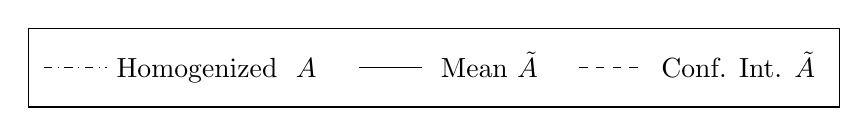
\begin{tikzpicture}
		\draw (0,4.5) -- (10.3,4.5) -- (10.3,5.5) -- (0,5.5) -- (0,4.5);
		\draw[style=dashdotted] (.2,5) -- (1,5) node[right]{Homogenized \vphantom{$\tilde A$} $A$};
		\draw[] (4.2,5) -- (5,5) node[right]{\vphantom{g} Mean $\tilde A$};
		\draw[style=dashed] (7,5) -- (7.8,5) node[right]{\vphantom{g} Conf. Int. $\tilde A$};
	\end{tikzpicture} 

	\vspace{0.5cm}
	\centering
	\begin{tabular}{cccc}
		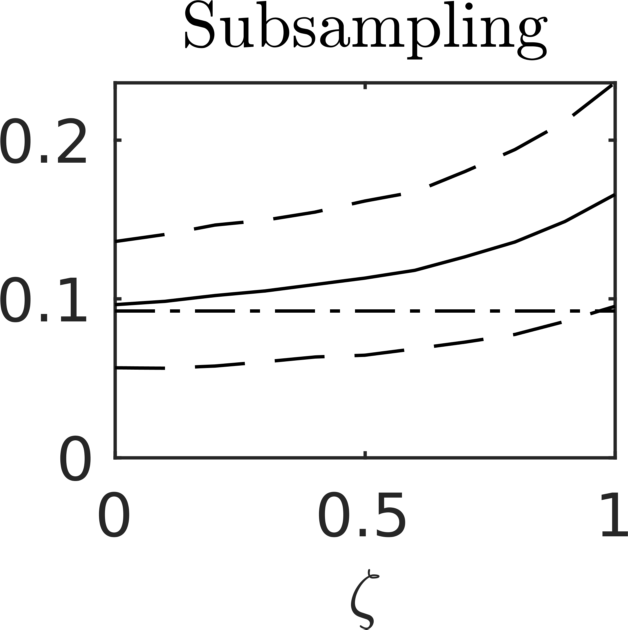
\includegraphics[]{Figures/A_sub_s4.png} & 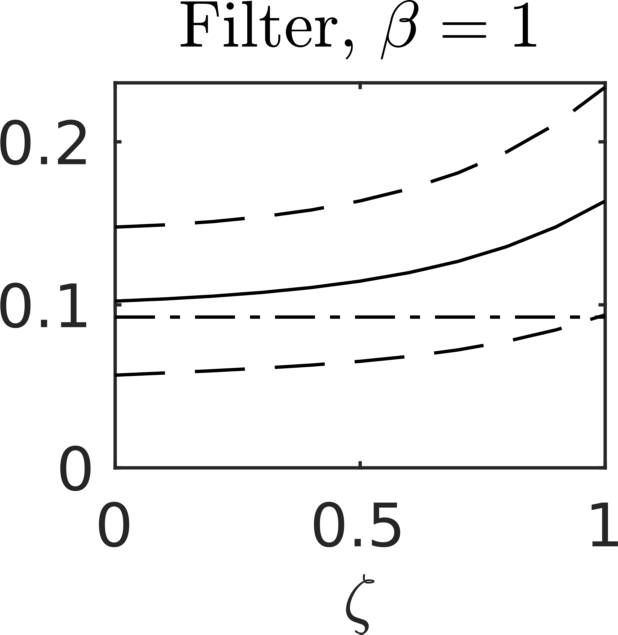
\includegraphics[]{Figures/A_filt_s4_b1.png} &
		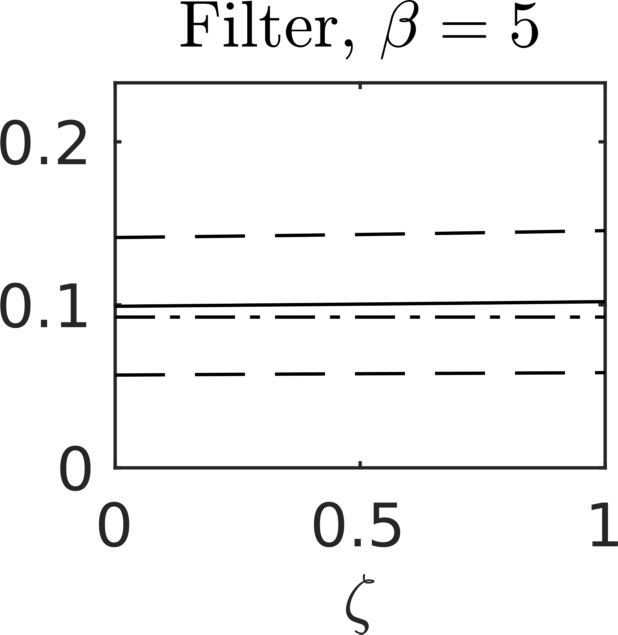
\includegraphics[]{Figures/A_filt_s4_b5.png} & 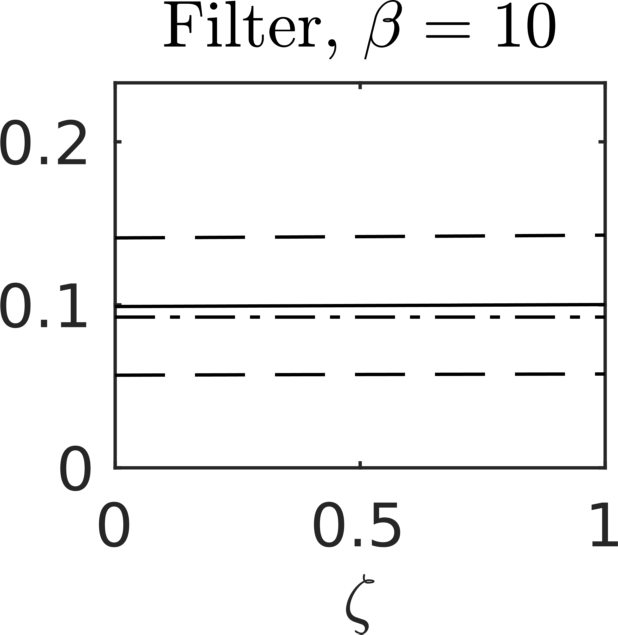
\includegraphics[]{Figures/A_filt_s4_b10.png}
	\end{tabular}	
	\caption{Results for $\sigma = 0.4$.}
	\end{subfigure}

	\vspace{0.5cm}
	\begin{subfigure}{\linewidth}
		\centering
		\begin{tabular}{cccc}
			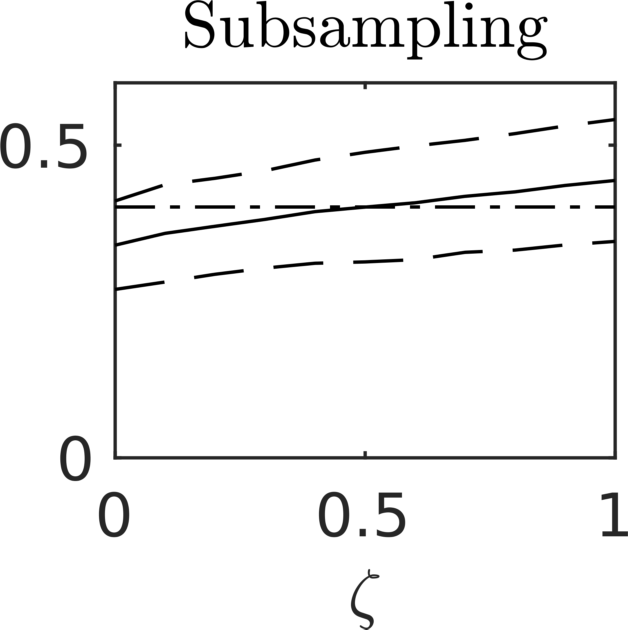
\includegraphics[]{Figures/A_sub_s7.png} & 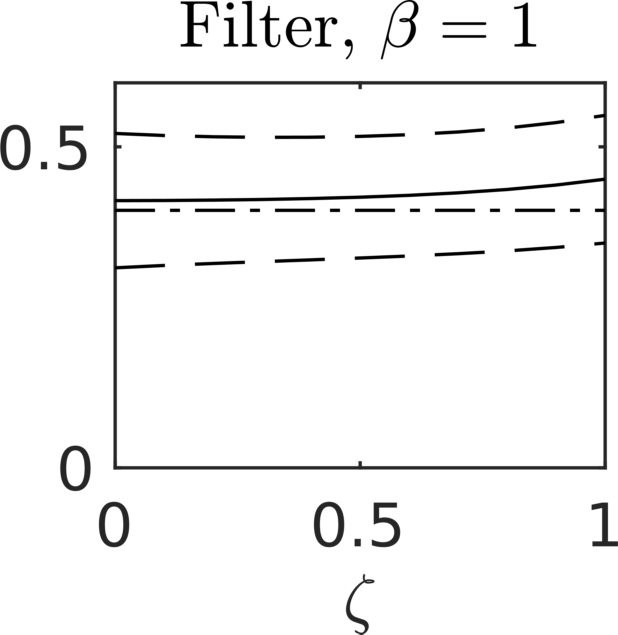
\includegraphics[]{Figures/A_filt_s7_b1.png} &
			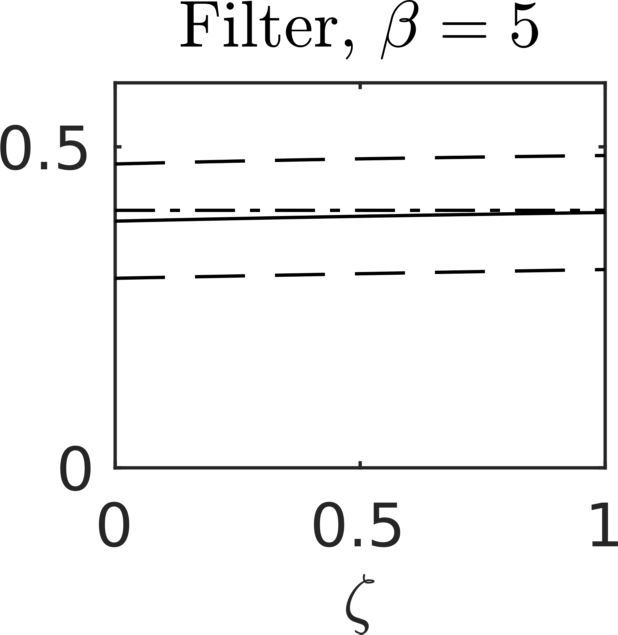
\includegraphics[]{Figures/A_filt_s7_b5.png} & 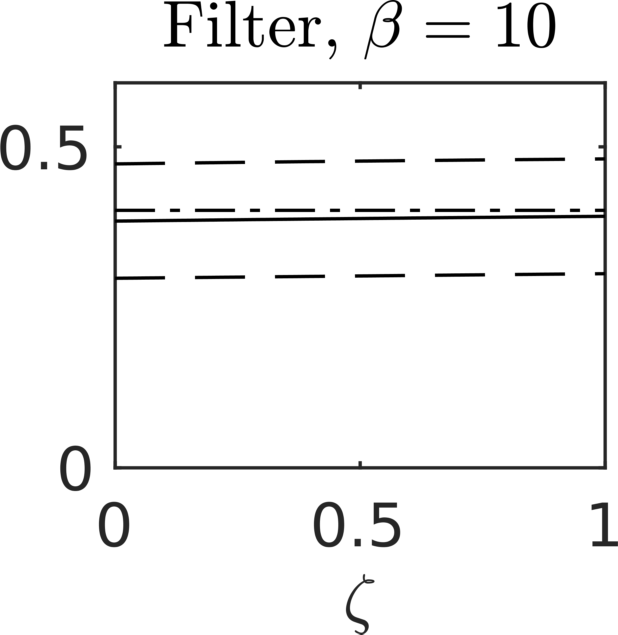
\includegraphics[]{Figures/A_filt_s7_b10.png}
		\end{tabular}	
	\caption{Results for $\sigma = 0.7$.}
	\end{subfigure}

	\vspace{0.5cm}
	\begin{subfigure}{\linewidth}
		\centering
		\begin{tabular}{cccc}
			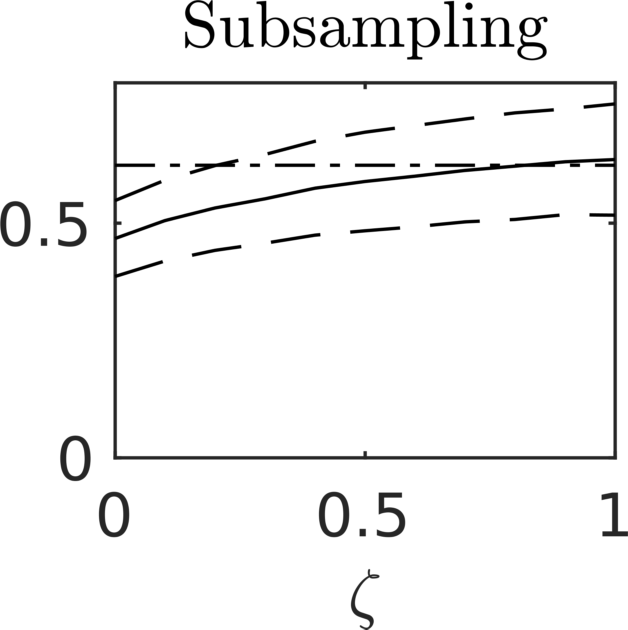
\includegraphics[]{Figures/A_sub_s10.png} & 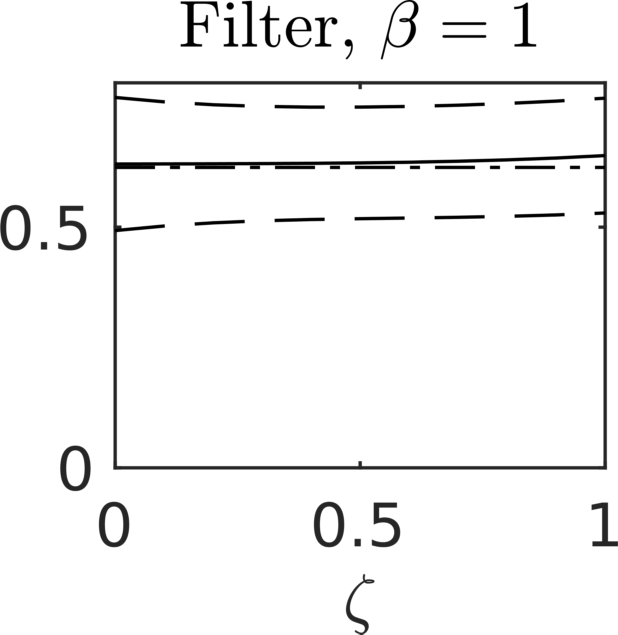
\includegraphics[]{Figures/A_filt_s10_b1.png} &
			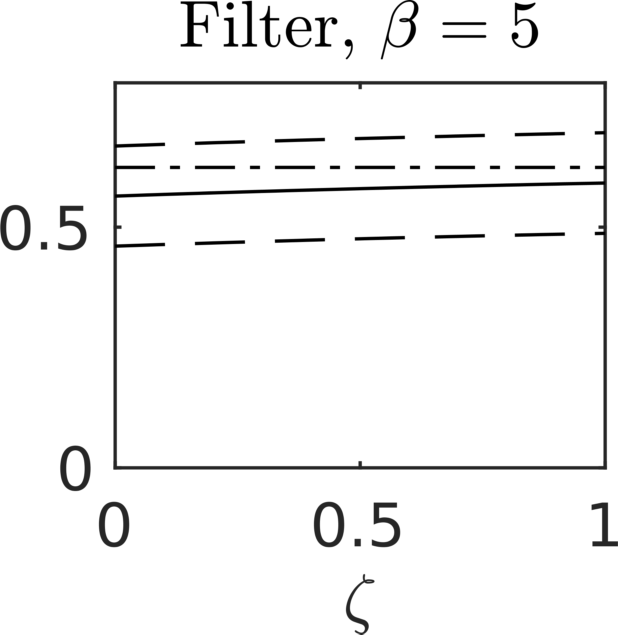
\includegraphics[]{Figures/A_filt_s10_b5.png} & 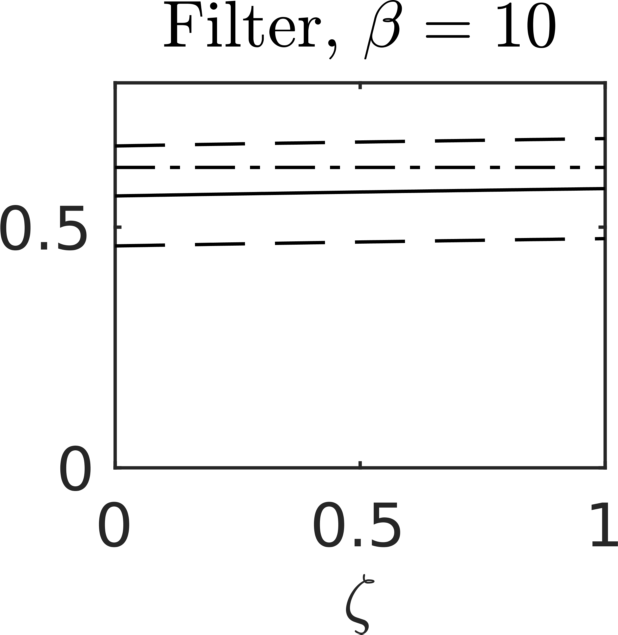
\includegraphics[]{Figures/A_filt_s10_b10.png}
		\end{tabular}	
		\caption{Results for $\sigma = 1$.}
	\end{subfigure}
	\caption{Summary of results for the Ornstein--Uhlenbeck process with $\epl=0.05$.}
	\label{fig:Result_OU}
\end{figure}

\begin{figure}[t]
	\begin{subfigure}{\linewidth}
		\centering
		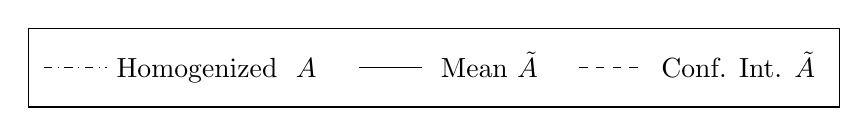
\begin{tikzpicture}
		\draw (0,4.5) -- (10.3,4.5) -- (10.3,5.5) -- (0,5.5) -- (0,4.5);
		\draw[style=dashdotted] (.2,5) -- (1,5) node[right]{Homogenized \vphantom{$\tilde A$} $A$};
		\draw[] (4.2,5) -- (5,5) node[right]{\vphantom{g} Mean $\tilde A$};
		\draw[style=dashed] (7,5) -- (7.8,5) node[right]{\vphantom{g} Conf. Int. $\tilde A$};
		\end{tikzpicture} 
		
		\vspace{0.5cm}
		\centering
		\begin{tabular}{cccc}
			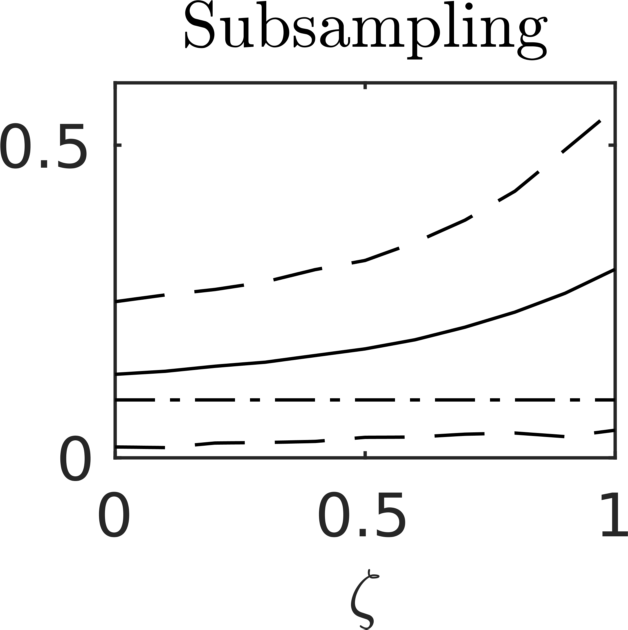
\includegraphics[]{Figures/A2_sub_s4.png} & 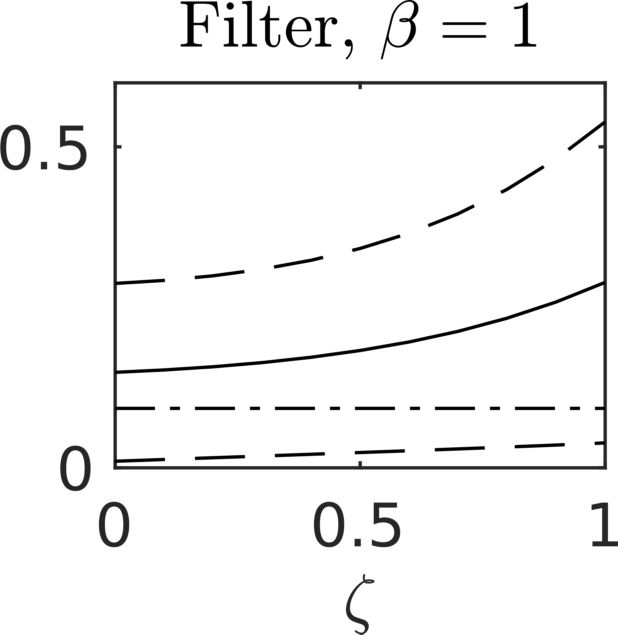
\includegraphics[]{Figures/A2_filt_s4_b1.png} &
			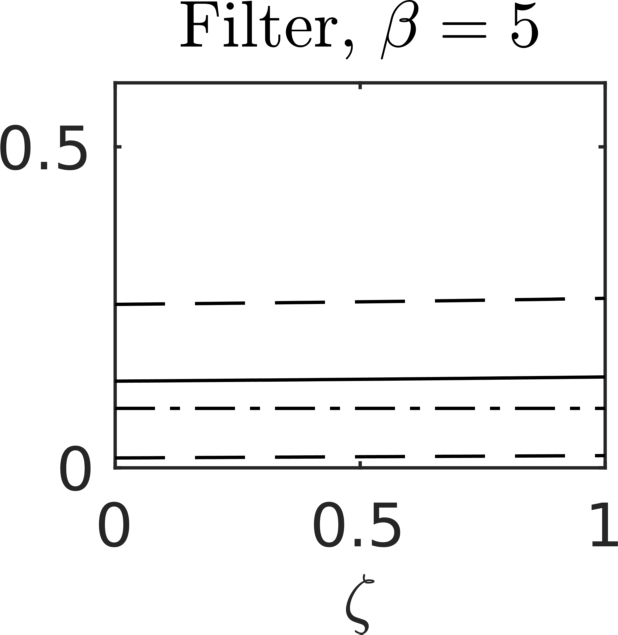
\includegraphics[]{Figures/A2_filt_s4_b5.png} & 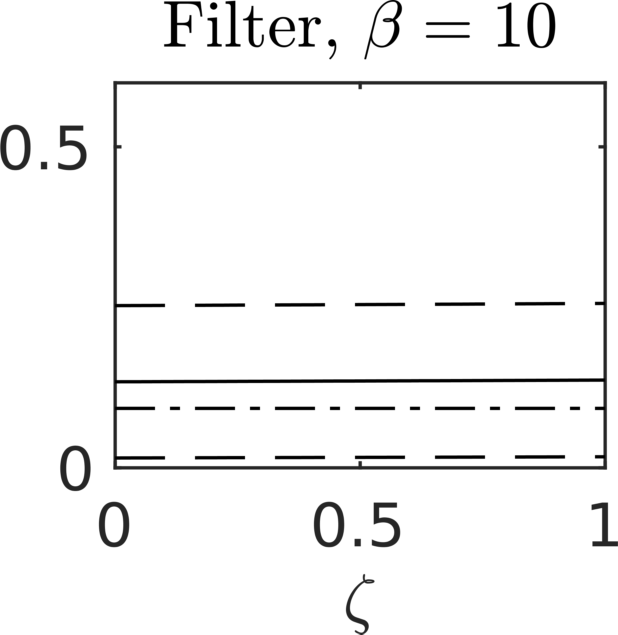
\includegraphics[]{Figures/A2_filt_s4_b10.png}
		\end{tabular}	
		\caption{Results for $\sigma = 0.4$.}
	\end{subfigure}
	
	\vspace{0.5cm}
	\begin{subfigure}{\linewidth}
		\centering
		\begin{tabular}{cccc}
			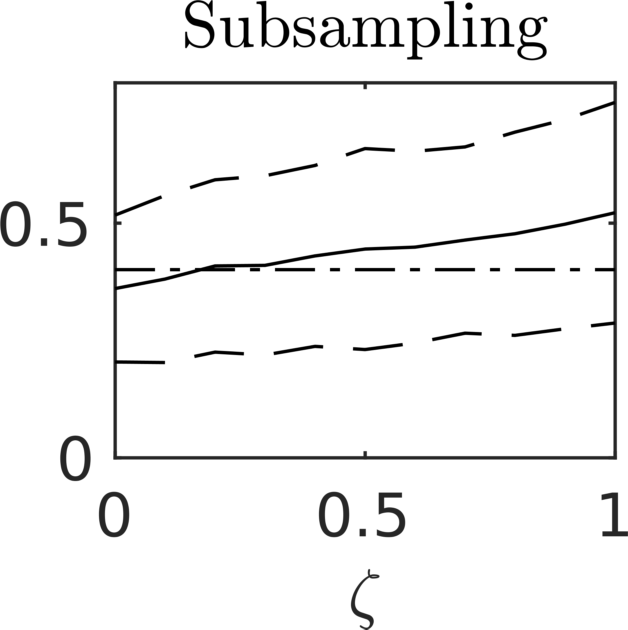
\includegraphics[]{Figures/A2_sub_s7.png} & 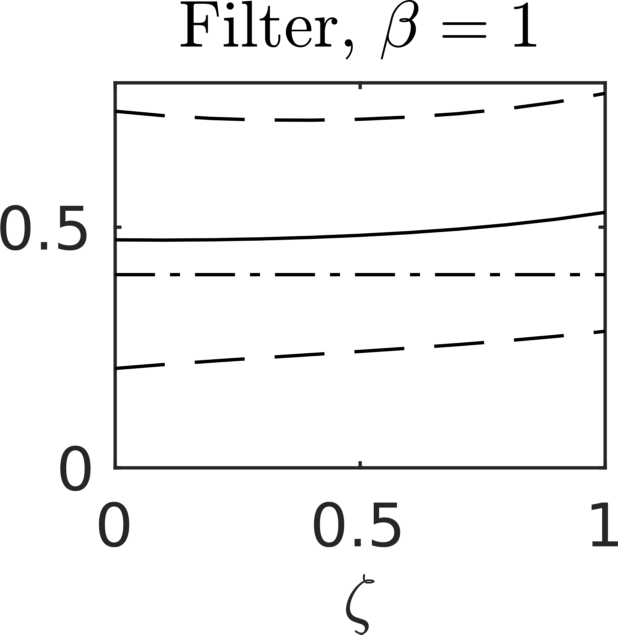
\includegraphics[]{Figures/A2_filt_s7_b1.png} &
			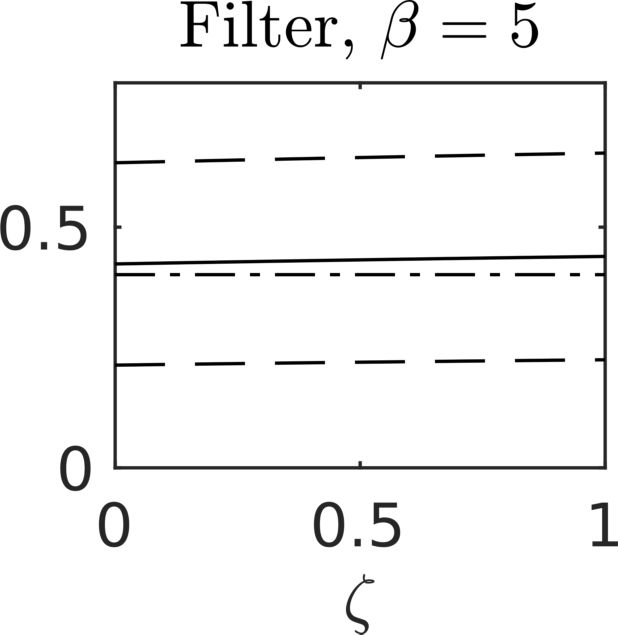
\includegraphics[]{Figures/A2_filt_s7_b5.png} & 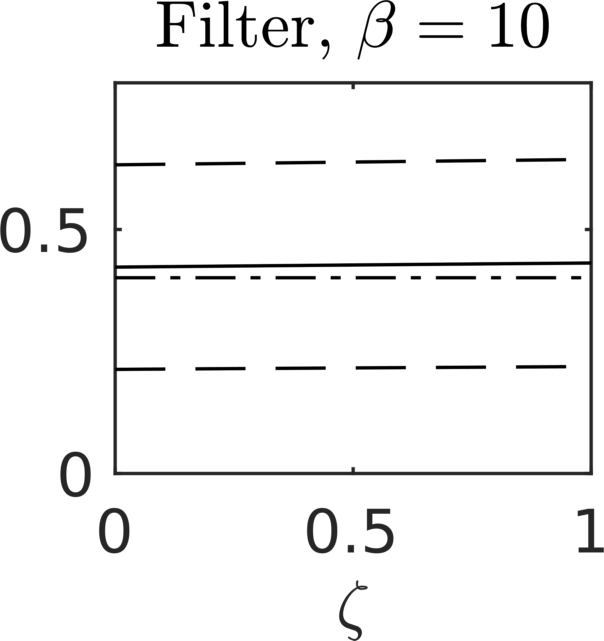
\includegraphics[]{Figures/A2_filt_s7_b10.png}
		\end{tabular}	
		\caption{Results for $\sigma = 0.7$.}
	\end{subfigure}
	
	\vspace{0.5cm}
	\begin{subfigure}{\linewidth}
		\centering
		\begin{tabular}{cccc}
			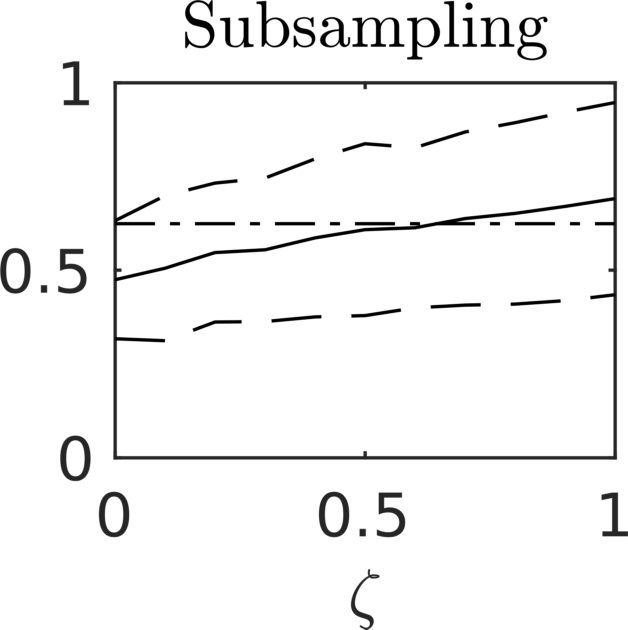
\includegraphics[]{Figures/A2_sub_s10.png} & 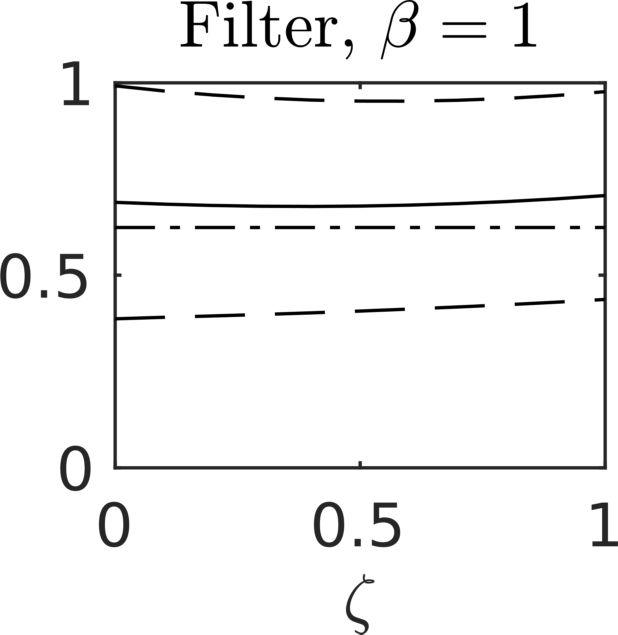
\includegraphics[]{Figures/A2_filt_s10_b1.png} &
			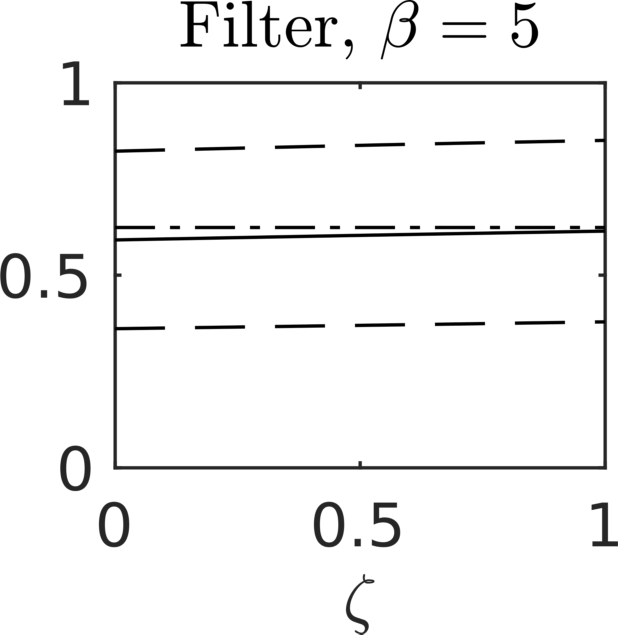
\includegraphics[]{Figures/A2_filt_s10_b5.png} & 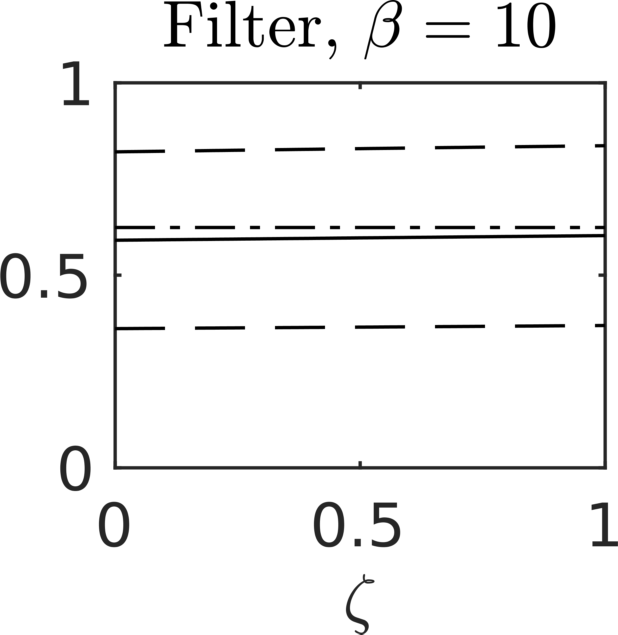
\includegraphics[]{Figures/A2_filt_s10_b10.png}
		\end{tabular}	
		\caption{Results for $\sigma = 1$.}
	\end{subfigure}
	\caption{Summary of results for the Ornstein--Uhlenbeck process with $\epl=0.1$.}
	\label{fig:Result_OU_2}
\end{figure}

\section{Current ideas}

\subsection{Stratonovich}
The numerator of the estimator $\hat A$ seems to converge to the Stratonovich integral of the multiscale process when the filter is applied. In particular, I observed numerically that (can it be proved?)
\begin{equation}
	\int_0^T V'(Z^{\epl,k}_t) \dd Z^{\epl,k}_t \approx \int_0^T V'(X^\epl_t) \circ \d X^\epl_t = V(X_T^\epl) - V(X_0^\epl).
\end{equation}
Therefore, one can compute the estimator 
\begin{equation}
	\widehat A_T (Z^{\epl,k}_{0:T}) = - \frac{\int_0^T V'(Z^{\epl,k}_t) \dd Z^{\epl,k}_t - \hat \Sigma \int_0^T V''(Z_t^{\epl,\kappa}) \dd t}{\int_0^T V'(Z^{\epl,k}_t)^2 \dd t},
\end{equation}
which accounts for the conversion of Itô--Stratonovich integrals. 

\begin{remark} I just noticed that since
	\begin{equation}
		\E^{\mu^\epl}(V(X_T^\epl) - V(X_0^\epl)) = 0,
	\end{equation}
	then this estimator is approximately equal to $\widetilde A$. Therefore, numerical experiments are given in the following section.
	
\end{remark}

\subsection{Estimator $\widetilde A$}
We consider the estimator
\begin{equation}
	\widetilde A_T(Z_{0:T}^{\epl,k}) = \widehat \Sigma \, \frac{\int_0^T  V''(Z_t^\epl) \dd t}{\int_0^T V'(Z_t^\epl)^2 \dd t}.
\end{equation}
For this estimator to be unbiased, it is necessary to have the two following ingredients
\begin{itemize}[label=-]
	\item An unbiased estimator $\widehat \Sigma$ of $\Sigma$,
	\item the process $Z_t^{\epl,k}$ should have the invariant distribution of the homogenized process as a limit invariant distribution.
\end{itemize}
These two issues are treated respectively in Section \ref{sec:Sigma} and \ref{sec:Ergodic}. Therefore, we can argue that (to be proved)
\begin{equation}
	\lim_{T\to\infty}\lim_{\epl \to 0} \widetilde A(Z_t^{\epl,k}) = A.
\end{equation}
Numerically, this seem to hold, but the behaviour of the estimator seems to give no better results (qualitatively) than the estimator obtained with subsampling. Results of test with $V(x) = x^2/2$ (Ornstein--Uhlenbeck) and with a quartic potential $V(x) = x^4 / 4$ can be found in Figure \ref{fig:OU} and Figure \ref{fig:Quartic}. In both figures, we plot the histogram and estimated density over $1000$ realization of the MLE for both the filter and the subsampling method. For these experiments, the parameter values where $\alpha = 1$, $\sigma = 0.5$, $\epl=0.1$, $T = \epl^{-\gamma}$ with $\gamma = 1.5$ and I employed the exponential filter of Example \ref{ex:expKernel}.

%\section{Numerical experiments}
%
%\subsection{Bistable potential}
%
%\subsection{Real(istic) data?}

\begin{appendices}

\section{Proofs}

\subsection*{Proof of lemma \ref{lem:diffusionLemma}}

We have
\begin{equation}
\E I(t)^2 = 2 \Sigma \int_0^t \int_0^t \partial_s k^\epl(t, s) \partial_r k^\epl(t, r) \sqrt{(t- s)(t-r)} \E \xi_{t,s}\xi_{t,r} \dd r \dd s.
\end{equation}
Let us remark that $\sqrt{t-s}\, \xi_{t,s} = \widetilde W(t) - \widetilde W(s)$, where $\widetilde W$ is a standard Brownian motion. Therefore 
\begin{equation}
\begin{aligned}
\E I(t)^2 &= 2\Sigma \int_0^t \int_0^t \partial_s k^\epl(t, s) \partial_r k^\epl(t, r) (t-s-r+\min\{s,r\}) \dd r \dd s \\
&= 
\begin{aligned}[t]
& 2\Sigma \int_0^t \int_0^s \partial_s k^\epl(t, s) \partial_r k^\epl(t, r) (t-s) \dd r \dd s \\
&+ 2\Sigma \int_0^t \int_s^t \partial_s k^\epl(t, s) \partial_r k^\epl(t, r) (t-r) \dd r \dd s 
\end{aligned}
\end{aligned}
\end{equation}
By straightforward calculations, one can show that
\begin{equation}
\E I(t)^2 = 2\Sigma \int_0^t \left(k^\epl(t,s) - k^\epl(t,0)\right)^2 \dd s.
\end{equation}
Since
\begin{equation}
k^\epl(t, s) = C_\beta\frac1{\delta^{1/\beta}} e^{-(t-s)^\beta / \delta},
\end{equation}
where $C_\beta = \beta \Gamma(1/\beta)^{-1}$, we have the explicit formula
\begin{equation}
\begin{aligned}
\frac1{2\Sigma }\E I(t)^2 &= \beta\Gamma\left(\frac1\beta\right)^{-2} \left((2\delta)^{-1/\beta}\gamma\left(\frac1\beta, \frac{2t^\beta}{\delta}\right) -2 \delta^{-1/\beta}\gamma\left(\frac1\beta, \frac{t^\beta}{\delta}\right)e^{-t^\beta/\delta} + \beta t \delta^{-2/\beta} e^{-2t^\beta/\delta}\right).
\end{aligned}
\end{equation}
Moreover, considering $\bar k \defeq k^\epl(t, t) = \beta \Gamma(1/\beta)^{-1}\delta^{-1/\beta}$, we have
\begin{equation}
\E I(t)^2 = 2 \Sigma \bar k  \left( C_1 - C_2 e^{-t^\beta/\delta} + C_3 \delta^{-1/\beta} t e^{-2t^\beta/\delta}\right),
\end{equation}
where 
\begin{equation}\label{eq:LemmaDiffusionConstants}
\begin{aligned}
C_1 &= 2^{-1/\beta} \Gamma(1/\beta)^{-1} \gamma\left(\frac1\beta, \frac{2t^\beta}{\delta}\right), \\
C_2 &= 2 \gamma\left(\frac1\beta, \frac{t^\beta}{\delta}\right),\\
C_3 &= \beta \Gamma(1/\beta)^{-1},
\end{aligned}
\end{equation}
which is the desired result since $C_1$, $C_2$ and $C_3$ are bounded independently of $\delta$ and $t$. \qed

\subsection*{Proof of Lemma \ref{lem:diffusionLemma2}}
We write
\begin{equation}
\begin{aligned}
I - \widehat I = &\int_{\bar t}^{\bar t+h} \int_{\bar{t}}^t \partial_t k^\epl(t, s) \sqrt{2\Sigma(t-s)} \, \xi_{t,s} \dd s \dd t\\
+ &\int_{\bar t}^{\bar t+h} \int_0^t \left( \partial_t k^\epl(t, s) \sqrt{2\Sigma(t-s)} \, \xi_{t,s}  - \partial_t k^\epl(\bar t, s) \sqrt{2\Sigma(\bar t-s)} \, \xi_{\bar t,s} \right)\dd s \dd t\\
&\eqdef R_1 + R_2.
\end{aligned}
\end{equation}
Young's inequality yields
\begin{equation}
\E\abs{I-\widehat I}^2 \leq 2\E\abs{R_1}^2 + 2\E\abs{R_2}^2.
\end{equation}
We bound $R_1$ and $R_2$ separately. First, due to the Cauchy--Schwarz inequality and since $\E \xi_{t,s}^2 = 1$, we have
\begin{equation}
\E \abs{R_1}^2 \leq 2\Sigma h^2 \int_{\bar t}^{\bar t+h} \int_{\bar{t}}^t (\partial_t k^\epl(t, s))^2  (t-s) \dd s \dd t.
\end{equation}
Let us remark that
\begin{equation}
	\max_{0\leq s \leq t} \left( -\partial_t k^\epl(t,s) \right) \leq	C_\beta \frac1{\delta^{1/\beta}} \left(\frac{\beta - 1}{\beta}\right)^{(\beta - 1)/\beta} e^{-(\beta-1)/\beta} \eqdef \frac{\widehat C_\beta}{\delta^{1/\beta}},
\end{equation}
so that
\begin{equation}
\E \abs{R_1}^2 \leq - \frac{2\Sigma  \widehat C_\beta h^2}{\delta^{1/\beta}} \int_{\bar{t}}^{\bar t + h}\int_{\bar t}^t -\partial_t k^\epl(t, s)(t-s) \dd s \dd t.
\end{equation}
For the inner integral, exploiting Assumption \ref{as:kern}.\ref{as:kernDivFree}, we have
\begin{equation}
\begin{aligned}
\int_{\bar t}^t -\partial_t k^\epl(t, s)(t-s) \dd s &= \int_{\bar t}^t \partial_s k^\epl(t, s)(t-s)\\
&= -k^\epl(t, \bar t)(t - \bar t) + \int_{\bar t}^t k^\epl(t, s) \dd s \\
&\leq (t - \bar t) \left(k^\epl(t, t) - k^\epl(t, \bar t)\right).
\end{aligned}
\end{equation}
Hence, replacing the definition of $k^\epl(t, s)$ and noticing that $k^\epl(t, \bar t) \geq k^\epl(\bar t+h, \bar t)$ for all $t \in [\bar t, \bar t + h]$, we obtain
\begin{equation}
\begin{aligned}
\E \abs{R_1}^2 &\leq \frac{2\Sigma \widehat C_\beta h^2}{\delta^{1/\beta}}\int_{\bar t}^{\bar t + h}(t - \bar t) \left(k^\epl(t, t) - k^\epl(t, \bar t)\right) \dd t\\
&\leq \frac{\Sigma C_\beta \widehat C_\beta h^4 }{\delta^{2/\beta}}\left(1 - e^{-h^\beta / \delta}\right) \leq \frac{\Sigma C_\beta \widehat C_\beta h^5}{\delta^{(\beta+2)/\beta}} ,
\end{aligned}
\end{equation}
where we exploited the inequality $1-e^{-x} \leq x$. We now proceed bounding $R_2$. The Cauchy--Schwarz inequality implies
\begin{equation}
\begin{aligned}
\E\abs{R_2}^2 &\leq 2 \Sigma h(\bar t + h)  \int_{\bar t}^{\bar t + h}\int_0^t 
\begin{aligned}[t]
&\left(\partial_t k^\epl(t, s)^2 (t-s)  + \partial_t k^\epl(\bar t, s)^2 (\bar t-s)\right.\\
&\left. -2 \partial_t k^\epl(t, s) \partial_t k^\epl(\bar t, s)(\bar t - s)\right) \dd s \dd t
\end{aligned}
\\
&= 2 \Sigma h(\bar t + h) \int_{\bar t}^{\bar t + h}\int_0^t 
\begin{aligned}[t]
&\left(\partial_t k^\epl(t, s)\left(\partial_t k^\epl(t, s)(t-s) -\partial_t k^\epl(\bar t, s)(\bar t - s)\right)\right.\\
&+ \left.  \partial_t k^\epl(\bar t, s)\left(\partial_t k^\epl(\bar t, s)- \partial_t k^\epl(t, s) \right)(\bar t - s) \right) \dd s \dd t.
\end{aligned}
\\
&\leq \frac{2 \Sigma h(\bar t + h)  \hat C_\beta}{\delta^{1/\beta}} 
\begin{aligned}[t]
&\left( \int_{\bar t}^{\bar t + h}\int_0^t \left(\partial_t k^\epl(\bar t, s)(\bar t - s) - \partial_t k^\epl(t, s)(t-s) \right) \dd s \dd t \right. \\
+ & \left. \int_{\bar t}^{\bar t + h}\int_0^t \left. \left(\partial_t k^\epl(\bar t, s) - \partial_t k^\epl(t, s)\right)(\bar t - s) \right) \dd s \dd t \right) 
\end{aligned}
\\
&\eqdef \frac{2 \Sigma h(\bar t + h)  \widehat C_\beta}{\delta^{1/\beta}}\left(R_{2,1} + R_{2,2}\right),
\end{aligned}
\end{equation}
where we employed the fact that $-\partial_t k^\epl(t,s) \leq -\widehat C_\beta \delta^{-1/\beta}$ for all $0 \leq s \leq t$ and for all $t \geq 0$. Due to Assumption \ref{as:kern} and to an integration by parts we can now compute
\begin{equation}
\begin{aligned}
	R_{2,1} &= \int_{\bar t}^{\bar t + h}\int_0^t \left(\partial_t k^\epl(\bar t, s)(\bar t - s) - \partial_t k^\epl(t, s)(t-s) \right) \dd s \dd t \\
	&= \int_{\bar t}^{\bar t + h} \int_0^t \left( \partial_s k^\epl(t, s)(t-s) - \partial_s k^\epl(\bar t, s)(\bar t - s) \right) \dd s \dd t \\
	&= \int_{\bar t}^{\bar t + h} \left(-k^\epl(t,0)t + \int_0^t k^\epl(t, s) \dd s + k^\epl(\bar t, t)(t - \bar t) + k^\epl(\bar t, 0)\bar t - \int_0^t k^\epl(\bar t, s) \dd s \right)\dd t\\
	&= \int_{\bar t}^{\bar t + h} \left(-k^\epl(t,0)t + 1 - \phi(t, \epl) + k^\epl(\bar t, t)(t - \bar t) + k^\epl(\bar t, 0)\bar t -\int_0^t k^\epl(\bar t, s) \dd s \right) \dd t.
\end{aligned}
\end{equation} 
Now, since $k^\epl(t, s)$ is a decreasing function of $t-s$, we have
\begin{equation}
\begin{aligned}
	\int_0^t k^\epl(\bar t, s) \dd s &= 1 - \phi(\bar t, \epl) + \int_{\bar t}^{t} k^\epl(\bar t, s) \dd s\\
	&\geq 1 - \phi(\bar t, \epl) + k^\epl(\bar t, t)(t - \bar t),
\end{aligned}
\end{equation}
so that
\begin{equation}
\begin{aligned}
	R_{2,1} \leq \int_{\bar t}^{\bar t + h} \left(k^\epl(\bar t, 0)\bar t - k^\epl(t,0)t + \phi(\bar t, \epl) - \phi(t, \epl) \right) \dd t.
\end{aligned}
\end{equation}
We can now bound the integrand of the expression above. First, since $t \geq \bar t$, we have
\begin{equation}
\begin{aligned}
	\phi(\bar t, \epl) - \phi(t, \epl) &= \Gamma(1/\beta)^{-1}\left(\gamma\left(\frac1\beta, \frac{t^\beta}{\delta}\right) - \gamma\left(\frac1\beta, \frac{\bar t^\beta}{\delta}\right) \right)\\
	&= \Gamma(1/\beta)^{-1} \int_{\bar t^\beta/\delta}^{t^\beta / \delta} s^{\frac1\beta - 1}e^{-s} \dd s\\
	&\leq  C_\beta \frac{e^{-\bar t^\beta / \delta} h}{\delta^{1/\beta}}.
\end{aligned}
\end{equation}
where we identified $C_\beta=\beta \Gamma(1/\beta)^{-1}$. Second, we have
\begin{equation}
\begin{aligned}
	k^\epl(\bar t, 0) \bar t - k^\epl(t, 0) t &= \frac{C_\beta}{\delta^{1/\beta}} \left(e^{-\bar t^\beta/\delta} \bar t - e^{-t^\beta / \delta} t\right) \\
	&\leq C_\beta\frac{e^{-\bar t^\beta / \delta}\bar t}{\delta^{1/\beta}}
\end{aligned}
\end{equation}
Finally, we combine the two inequalities above to get
\begin{equation}\label{eq:AppendixLemma_BoundR21}
	R_{2,1} \leq 2 C_\beta \frac{e^{-\bar t^\beta / \delta} (\bar t + h)h}{\delta^{1/\beta}}.
\end{equation}
We now consider $R_{2,2}$. We have
\begin{equation}
\begin{aligned}
	R_{2,2} &= \int_{\bar t}^{\bar t + h}\int_0^t \left(\partial_t k^\epl(\bar t, s) - \partial_t k^\epl(t, s)\right)(\bar t - s)  \dd s \dd t \\
	&= \int_{\bar t}^{\bar t + h}\int_0^t \left(\partial_t k^\epl(\bar t, s)(\bar t - s) - \partial_t k^\epl(t, s)(t-s) - \partial_t k^\epl(t, s)(\bar t - t)\right)\dd s \dd t \\
	&= \int_{\bar t}^{\bar t + h} 
	\begin{aligned}[t]
	&\left(\phi(\bar t, \epl) + \bar t k^\epl(\bar t, 0) + \int_{\bar t}^{t}\partial_t k^\epl(\bar t, s)(\bar t - s) \dd s \right.\\
	&- \left. \phi(t, \epl) - t k^\epl(t, 0) - \int_0^t \partial_t k^\epl(t, s)(\bar t - t) \dd s \right) \dd t
	\end{aligned}
\end{aligned}
\end{equation}
Let us remark that, due to the computations done for bounding $R_{2,1}$ above, we have
\begin{equation}
\begin{aligned}
	R_{2,2} \leq 2 C_\beta \frac{e^{-\bar t^\beta / \delta} (\bar t + h)h}{\delta^{1/\beta}} + \int_{\bar t}^{\bar t + h}\left(\int_{\bar t}^{t}\partial_t k^\epl(\bar t, s)(\bar t - s) \dd s -  \int_0^t \partial_t k^\epl(t, s)(\bar t - t) \dd s \right) \dd t.
\end{aligned}
\end{equation}
One can show that the second term in the inequality above is negative, and therefore that
\begin{equation}\label{eq:AppendixLemma_BoundR22}
	R_{2,2} \leq  2 C_\beta \frac{e^{-\bar t^\beta / \delta} (\bar t + h)h}{\delta^{1/\beta}}.
\end{equation}
Regrouping \eqref{eq:AppendixLemma_BoundR21} and \eqref{eq:AppendixLemma_BoundR22} we get
\begin{equation}
	\E\abs{R_2}^2 \leq 8 \Sigma C_\beta \widehat C_\beta \frac{e^{-\bar t^\beta / \delta} (\bar t + h)^2h^2}{\delta^{2/\beta}}.
\end{equation} 
Finally
\begin{equation}
	\E\abs{I-\hat I}^2 \leq \Sigma C_\beta \widehat C_\beta \left( \frac{2h^5}{\delta^{(\beta+2)/\beta}} +  \frac{16e^{-\bar t^\beta / \delta} (\bar t + h)^2h^2}{\delta^{2/\beta}} \right),
\end{equation}
which proves the first bound. For the second bound, the Cauchy--Schwarz inequality implies
\begin{equation}
\begin{aligned}
	\E I^2 &\leq 2\Sigma h(\bar t + h) \int_{\bar t}^{\bar t + h} \int_0^t \left(\partial_t k^\epl(t,s)\right)^2 (t - s) \dd s \dd t\\
	&\leq \frac{2\Sigma h(\bar t + h) \widehat C_\beta}{\delta^{1/\beta}} \int_{\bar t}^{\bar t + h} (1 - \phi(t, \epl) - tk^\epl(t, 0) )\dd t\\
	&\leq \frac{2\Sigma h^2(\bar t + h) \widehat C_\beta}{\delta^{1/\beta}},
\end{aligned}
\end{equation}
which proves the desired result.
\qed

\end{appendices}


\bibliographystyle{siam}
\bibliography{../../anmc}
\end{document}  